
\documentclass[12pt,reqno]{amsart}
%%%%%%%%%%%%%%%%%%%%%%%%%%%%%%%%%%%%%%%%%%%%%%%%%%%%%%%%%%%%%%%%%%%%%%%%%%%%%%%%%%%%%%%%%%%%%%%%%%%%%%%%%%%%%%%%%%%%%%%%%%%%%%%%%%%%%%%%%%%%%%%%%%%%%%%%%%%%%%%%%%%%%%%%%%%%%%%%%%%%%%%%%%%%%%%%%%%%%%%%%%%%%%%%%%%%%%%%%%%%%%%%%%%%%%%%%%%%%%%%%%%%%%%%%%%%
\usepackage{mathtools}
\usepackage{amsfonts}
\usepackage[utf8]{inputenc}
\usepackage{amsmath,amssymb,amsthm}
\usepackage{float}
\usepackage{array}
\usepackage{graphicx}
\usepackage{setspace}
\usepackage{xcolor}
\usepackage{enumitem}
\usepackage[margin=17mm]{geometry}
\usepackage{tikz}
\usepackage{fancyvrb}
\usepackage{fancyhdr}
\usepackage{titlesec,titletoc}
\usepackage[colorlinks=true,linkcolor=blue,citecolor=green,urlcolor=magenta]{hyperref}
\usepackage{aliascnt}
\usepackage[nameinlink]{cleveref}
\usepackage{listings}
\usepackage{booktabs}

\setcounter{MaxMatrixCols}{10}
%TCIDATA{OutputFilter=LATEX.DLL}
%TCIDATA{Version=5.50.0.2960}
%TCIDATA{<META NAME="SaveForMode" CONTENT="1">}
%TCIDATA{BibliographyScheme=Manual}
%TCIDATA{LastRevised=Tuesday, November 24, 2026 17:36:55}
%TCIDATA{<META NAME="GraphicsSave" CONTENT="32">}

\setlength{\tabcolsep}{3pt}
\renewcommand{\arraystretch}{1.35}
\renewcommand{\tablename}{$\textsf{Tab}$}
\setlength{\tabcolsep}{3pt}
\renewcommand{\arraystretch}{1.2}
\newcommand{\N}{\mathbb N}
\newcommand{\Z}{\mathbb Z}
\newcommand{\Q}{\mathbb Q}
\newcommand{\R}{\mathbb R}
\newcommand{\C}{\mathbb C}
\newcommand{\Np}{\N_{\ge1}}
\newcommand{\fl}[1]{\left\lfloor #1\right\rfloor}
\providecommand{\TEXTsymbol}[1]{#1}
\makeatletter
\newcommand{\SplitTableCaption}{\def\@captype{table}\caption}
\makeatother
\restylefloat{figure}
\hypersetup{pageanchor=false}
\makeatletter
\@ifundefined{theorem}{}{\let\theorem\relax}
\@ifundefined{definition}{}{\let\definition\relax}
\@ifundefined{lemma}{}{\let\lemma\relax}
\@ifundefined{corollary}{}{\let\corollary\relax}
\@ifundefined{proposition}{}{\let\proposition\relax}
\@ifundefined{remark}{}{\let\remark\relax}
\@ifundefined{statement}{}{\let\statement\relax}
\makeatother
\DeclareUnicodeCharacter{03B9}{\ensuremath{\iota}}
\DeclareUnicodeCharacter{2200}{\ensuremath{\forall}}
\DeclareUnicodeCharacter{2203}{\ensuremath{\exists }}
\DeclareUnicodeCharacter{2208}{\ensuremath{\in}}
\DeclareUnicodeCharacter{2218}{\ensuremath{\circ}}
\DeclareUnicodeCharacter{2264}{\ensuremath{\leq}}
\DeclareUnicodeCharacter{2265}{\ensuremath{\geq}}
\DeclareUnicodeCharacter{2192}{\ensuremath{\to}}
\DeclareUnicodeCharacter{21A6}{\ensuremath{\mapsto}}
\DeclareUnicodeCharacter{2260}{\ensuremath{\neq}}
\DeclareUnicodeCharacter{00D7}{\ensuremath{\times}}
\DeclareUnicodeCharacter{2115}{\ensuremath{\mathbb{N}}}
\DeclareUnicodeCharacter{211D}{\ensuremath{\mathbb{R}}}
\DeclareUnicodeCharacter{27E8}{\ensuremath{\langle}}
\DeclareUnicodeCharacter{27E9}{\ensuremath{\rangle}}
\providecommand{\period}{\,\allowbreak}
\newcommand{\pagenumside}{C}
\newlength{\pageNumberOffset}
\setlength{\pageNumberOffset}{0pt}
\newcommand{\PagenumSideC}{C}
\newcommand{\applypagehead}[1]{\expandafter\fancyhead\expandafter[\pagenumside]{#1}\ifx\pagenumside\PagenumSideC\else\ifdim\pageNumberOffset=0pt\else\expandafter\fancyheadoffset\expandafter[\pagenumside]{\pageNumberOffset}\fi\fi}
\newcommand{\applypagefoot}[1]{\expandafter\fancyfoot\expandafter[\pagenumside]{#1}\ifx\pagenumside\PagenumSideC\else\ifdim\pageNumberOffset=0pt\else\expandafter\fancyfootoffset\expandafter[\pagenumside]{\pageNumberOffset}\fi\fi}
\pagestyle{fancy}
\fancyhf{}
\applypagehead{\thepage}
\renewcommand{\headrulewidth}{0pt}
\renewcommand{\footrulewidth}{0pt}
\fancypagestyle{plain}{\fancyhf{}\applypagehead{\thepage}\renewcommand{\headrulewidth}{0pt}}
\setlength{\arraycolsep}{1.5pt}
\setlength{\tabcolsep}{1.5pt}
\renewcommand{\arraystretch}{1.0}
\setlength{\arrayrulewidth}{0.4pt}
\setlength{\doublerulesep}{1pt}
\setlength{\extrarowheight}{0pt}
\newcolumntype{C}{>{\centering\arraybackslash\scriptsize}m{40pt}}
\newcolumntype{R}{>{\centering\arraybackslash\scriptsize}m{2.5cm}}
\newcolumntype{L}{>{\centering\arraybackslash\scriptsize}m{10.5cm}}
\fvset{frame=lines,framerule=0.7pt,rulecolor=\color{blue!60!black},framesep=2pt,fontsize=\scriptsize,xleftmargin=4pt,xrightmargin=4pt}
\RecustomVerbatimEnvironment{verbatim}{Verbatim}{}
\DefineVerbatimEnvironment{verbatimbox}{Verbatim}{frame=single,framerule=0.7pt,rulecolor=\color{blue!60!black},framesep=2pt,fontsize=\scriptsize,xleftmargin=4pt,xrightmargin=4pt}
\makeatletter
\def\@setsubjclass{\ifx\@subjclass\@empty\else\@subjclass\fi}
\makeatother
\subjclass{\textbf{2020 Mathematics Subject Classification.}\,Primary 26A06; Secondary 26A42.}
\keywords{fundamental theorem of calculus, Riemann integration, Darboux sums, mean value theorem, typed proofs}
\renewcommand{\abstractname}{\fontsize{9}{11}\selectfont Abstract}
\newcommand{\abstractfont}{\normalfont\fontsize{8}{10}\selectfont}
\newcommand{\abstractheadingsep}{\vspace{0.5em}}
\makeatletter
\renewenvironment{abstract}{\ifx\maketitle\relax\ClassWarning{\@classname}{Abstract should precede\protect\maketitle\space in AMS document classes reported}\fi\global\setbox\abstractbox=\vtop \bgroup\abstractfont{\centering\abstractname\par}\abstractheadingsep\list{}{\labelwidth\z@\leftmargin3pc \rightmargin\leftmargin\listparindent\normalparindent \itemindent\z@\parsep\z@ \@plus\p@\let\fullwidthdisplay\relax}\item\relax}{\endlist\egroup\ifx\@setabstract\relax \@setabstracta \fi}
\makeatother
\setcounter{secnumdepth}{3}
\newcommand{\SecAbove}{1.0ex plus 0.3ex minus 0.1ex}
\newcommand{\SecBelow}{0pt}
\newcommand{\SubsecAbove}{0.8ex plus 0.2ex minus 0.1ex}
\newcommand{\SubsecBelow}{0pt}
\newcommand{\SubsubsecAbove}{0.6ex plus 0.2ex minus 0.1ex}
\newcommand{\SubsubsecBelow}{0pt}
\makeatletter
\titleformat{\section}{\normalfont\fontsize{16}{18}\selectfont\bfseries}{\thesection.}{0.5em}{}
\titleformat{\subsection}{\normalfont\fontsize{14}{16}\selectfont\bfseries}{\thesubsection.}{0.5em}{}
\titleformat{\subsubsection}{\normalfont\fontsize{12}{14}\selectfont\bfseries}{\thesubsubsection.}{0.5em}{}
\titlespacing*{\section}{\z@}{\SecAbove}{\SecBelow}
\titlespacing*{\subsection}{\z@}{\SubsecAbove}{\SubsecBelow}
\titlespacing*{\subsubsection}{\z@}{\SubsubsecAbove}{\SubsubsecBelow}
\makeatother
\newcounter{axctr}\newcounter{posctr}
\newcounter{lemctr}\newcounter{thmctr}\newcounter{asserctr}\newcounter{corctr}
\renewcommand{\theaxctr}{\arabic{axctr}}
\renewcommand{\theposctr}{\arabic{posctr}}
\renewcommand{\thelemctr}{\arabic{lemctr}}
\renewcommand{\thethmctr}{\arabic{thmctr}}
\renewcommand{\theasserctr}{\arabic{asserctr}}
\renewcommand{\thecorctr}{\arabic{corctr}}
\renewcommand{\theHaxctr}{\thesection.\arabic{axctr}}
\renewcommand{\theHposctr}{\thesection.\arabic{posctr}}
\renewcommand{\theHlemctr}{\thesection.\arabic{lemctr}}
\renewcommand{\theHthmctr}{\thesection.\arabic{thmctr}}
\renewcommand{\theHasserctr}{\thesection.\arabic{asserctr}}
\providecommand{\theHasser}{\theequation}
\renewcommand{\theHcorctr}{\thesection.\arabic{corctr}}
\newcommand{\swpax}[2]{\refstepcounter{axctr}\hypertarget{#1}{\mbox{\textbf{Ax\,\theaxctr}}}\label{#2}}
\newcommand{\swppos}[2]{\refstepcounter{posctr}\hypertarget{#1}{\mbox{\textbf{Pos\,\theposctr}}}\label{#2}}
\newcommand{\swplem}[2]{\refstepcounter{lemctr}\hyperlink{#1}{\mbox{\textbf{Lem\,\thelemctr}}}\label{#2}}
\newcommand{\swpthm}[2]{\refstepcounter{thmctr}\hyperlink{#1}{\mbox{\textbf{Thm\,\thethmctr}}}\label{#2}}
\newcommand{\swpcor}[2]{\refstepcounter{corctr}\hypertarget{#1}{\mbox{\textbf{Cor\,\thecorctr}}}\label{#2}}
\newcommand{\tagged}[2]{\hypertarget{#1}{\mbox{\textbf{#2}}}}
\newcommand{\autorefto}[2]{\hyperlink{#1}{#2}}
\newcommand{\mcite}[1]{\text{\cite{#1}}}
\newtheoremstyle{blueplain}{2pt plus 1pt minus 0.5pt}{1pt plus 0.5pt minus 0.3pt}{\itshape}{}{\bfseries\color{blue}}{.}{\newline}{\thmname{#1}\thmnumber{ #2}\thmnote{ {\bfseries\color{blue}(#3)}}}
\theoremstyle{blueplain}
\newtheorem{theorem}{Theorem}[section]
\newtheorem{lemma}{Lemma}[section]
\newtheorem{corollary}{Corollary}[section]
\newtheorem{proposition}{Proposition}[section]
\newtheorem{remark}{Remark}[section]
\newtheorem*{definition}{Definition}
\newtheorem{statement}{Statement}[section]
\definecolor{proofhead}{RGB}{11,83,148}
\definecolor{proofqed}{RGB}{204,0,0}
\renewcommand{\qedsymbol}{\textcolor{proofqed}{\ensuremath{\square}}}
\renewenvironment{proof}[1][Proof]{\par\noindent\textbf{\textcolor{proofhead}{#1.}}\par\nobreak}{\par\nobreak\hfill\qedsymbol}
\newenvironment{swpproof}[1][Proof]{\begin{proof}[#1]}{\end{proof}}
\renewcommand{\theHtheorem}{\thesection.\arabic{theorem}}
\renewcommand{\theHstatement}{\thesection.\arabic{statement}}
\providecommand{\axctrautorefname}{Axiom}
\providecommand{\posctrautorefname}{Postulate}
\providecommand{\lemctrautorefname}{Lemma}
\providecommand{\thmctrautorefname}{Theorem}
\providecommand{\asserctrautorefname}{Proposition}
\providecommand{\corctrautorefname}{Corollary}
\providecommand{\statementautorefname}{Statement}
\crefname{axctr}{axiom}{axioms}
\crefname{posctr}{postulate}{postulates}
\crefname{lemctr}{lemma}{lemmas}
\crefname{thmctr}{theorem}{theorems}
\crefname{asserctr}{proposition}{propositions}
\crefname{corctr}{corollary}{corollaries}
\Crefname{axctr}{Axiom}{Axioms}
\Crefname{posctr}{Postulate}{Postulates}
\Crefname{lemctr}{Lemma}{Lemmas}
\Crefname{thmctr}{Theorem}{Theorems}
\Crefname{asserctr}{Proposition}{Propositions}
\Crefname{corctr}{Corollary}{Corollaries}
\crefname{statement}{statement}{statements}
\Crefname{statement}{Statement}{Statements}
\crefname{section}{section}{sections}
\Crefname{section}{Section}{Sections}
\crefname{equation}{eq}{eqs}
\Crefname{equation}{Eq}{Eqs}
\crefformat{equation}{#2\textcolor{blue}{eq~#1}#3}
\Crefformat{equation}{#2\textcolor{blue}{Eq~#1}#3}
\newcounter{inq}
\renewcommand{\theinq}{\theequation}
\makeatletter
\renewcommand{\p@inq}{\p@equation}
\makeatother
\crefname{inq}{ineq}{inequalities}
\Crefname{inq}{Ineq}{Inequalities}
\crefformat{inq}{#2\textcolor{blue}{inequality~#1}#3}
\Crefformat{inq}{#2\textcolor{blue}{Inequality~#1}#3}
\crefmultiformat{inq}{#2\textcolor{blue}{inequalities~#1}#3}{\textcolor{blue}{ ,\,~#2#1#3}}{\textcolor{blue}{, #2#1#3}}{\textcolor{blue}{ ,\,~#2#1#3}}
\Crefmultiformat{inq}{#2\textcolor{blue}{Inequalities~#1}#3}{\textcolor{blue}{ ,\,~#2#1#3}}{\textcolor{blue}{, #2#1#3}}{\textcolor{blue}{ ,\,~#2#1#3}}
\makeatletter
\newenvironment{ineq}
{\begin{equation}\refstepcounter{inq}}
{\end{equation}}
\makeatother
\newcounter{type}
\renewcommand{\thetype}{\theequation}
\makeatletter
\renewcommand{\p@type}{\p@equation}
\makeatother
\crefname{type}{type}{types}
\Crefname{type}{Type}{Types}
\crefformat{type}{#2\textcolor{blue}{type~#1}#3}
\Crefformat{type}{#2\textcolor{blue}{Type~#1}#3}
\crefmultiformat{type}{#2\textcolor{blue}{types~#1}#3}{\textcolor{blue}{ ,\,~#2#1#3}}{\textcolor{blue}{, #2#1#3}}{\textcolor{blue}{ ,\,~#2#1#3}}
\Crefmultiformat{type}{#2\textcolor{blue}{Types~#1}#3}{\textcolor{blue}{ ,\,~#2#1#3}}{\textcolor{blue}{, #2#1#3}}{\textcolor{blue}{ ,\,~#2#1#3}}
\makeatletter
\newenvironment{type}
{\begin{equation}\refstepcounter{type}}
{\end{equation}}
\makeatother
\newcounter{asser}
\renewcommand{\theasser}{\theequation}
\makeatletter
\renewcommand{\p@asser}{\p@equation}
\makeatother
\crefname{asser}{Assertion}{assertions}
\Crefname{asser}{Assertion}{Assertions}
\crefformat{asser}{#2\textcolor{blue}{assertion~#1}#3}
\Crefformat{asser}{#2\textcolor{blue}{Assertion~#1}#3}
\crefmultiformat{asser}{#2\textcolor{blue}{assertions~#1}#3}{\textcolor{blue}{ ,\,~#2#1#3}}{\textcolor{blue}{, #2#1#3}}{\textcolor{blue}{ ,\,~#2#1#3}}
\Crefmultiformat{asser}{#2\textcolor{blue}{Assertions~#1}#3}{\textcolor{blue}{ ,\,~#2#1#3}}{\textcolor{blue}{, #2#1#3}}{\textcolor{blue}{ ,\,~#2#1#3}}
\makeatletter
\newenvironment{asser}
{\begin{equation}\refstepcounter{asser}}
{\end{equation}}
\makeatother
\newcommand{\thmref}[1]{\hyperref[#1]{Theorem~\ref*{#1}}}
\newcommand{\lemref}[1]{\hyperref[#1]{Lemma~\ref*{#1}}}
\newcommand{\corref}[1]{\hyperref[#1]{Corollary~\ref*{#1}}}
\newcommand{\propref}[1]{\hyperref[#1]{Proposition~\ref*{#1}}}
\makeatletter
\let\orig@maketitle\maketitle
\renewcommand{\maketitle}{\begingroup\let\MakeUppercase\@firstofone\let\uppercase\@firstofone\orig@maketitle\endgroup}
\newlength{\titleToAuthorSkip}
\newlength{\authorToAbstractSkip}
\setlength{\titleToAuthorSkip}{3pt plus 1pt minus 0.5pt}
\setlength{\authorToAbstractSkip}{4pt plus 1pt minus 0.5pt}
\renewcommand{\@maketitle}{\normalfont\normalsize\let\@makefnmark\relax\let\@thefnmark\relax\ifx\@empty\@subjclass\else\@footnotetext{\@setsubjclass}\fi\ifx\@empty\@keywords\else\@footnotetext{\@setkeywords}\fi\ifx\@empty\@thanks\else\@footnotetext{\@setthanks}\fi\@settitle\ifx\@empty\@authors\else\vspace{\titleToAuthorSkip}\@setauthors\fi\ifx\@empty\@date\else\vspace{3pt}\@setdate\fi\ifx\@empty\@abstract\else\vspace{\authorToAbstractSkip}\fi\@setabstract}
\makeatother
\makeatletter
\renewcommand{\encodingdefault}{OT1}
\makeatother
\renewcommand{\rmdefault}{cmr}
\renewcommand{\sfdefault}{cmss}
\renewcommand{\ttdefault}{cmtt}
\fontencoding{OT1}\fontfamily{cmr}\selectfont
\renewcommand{\contentsname}{\texorpdfstring{{\color{blue!60!black}\sffamily\Large\selectfont\bfseries Contents}}{Contents}}
\renewcommand{\seriesdefault}{\bfdefault}
\boldmath
\providecommand{\comma}{\allowbreak,\,}
\IfFileExists{tcilatex.tex}{\input{tcilatex}}{}
\makeatletter
\def\dudley@listtighten{  \setlength{\topsep}{0pt}  \setlength{\partopsep}{0pt}  \setlength{\itemsep}{1pt plus 0.5pt minus 0.3pt}  \setlength{\parsep}{0pt}  \setlength{\labelsep}{0.4em}}
\def\dudley@itemlabel{  \ifnum\@listdepth=\@ne \labelitemi
	\else\ifnum\@listdepth=\tw@ \labelitemii
	\else\ifnum\@listdepth=\thr@@ \labelitemiii
	\else \labelitemiv\fi\fi\fi}
\def\dudley@enumlabel{  \ifnum\@listdepth=\@ne \arabic{enumi}.
	\else\ifnum\@listdepth=\tw@ \alph{enumii}.
	\else\ifnum\@listdepth=\thr@@ \roman{enumiii}.
	\else \Alph{enumiv}.\fi\fi\fi}
\def\dudley@enumcounter{  \ifnum\@listdepth=\@ne \usecounter{enumi}  \else\ifnum\@listdepth=\tw@ \usecounter{enumii}  \else\ifnum\@listdepth=\thr@@ \usecounter{enumiii}  \else \usecounter{enumiv}\fi\fi\fi}
\makeatother
\setlength{\parindent}{0pt}
\setlength{\parskip}{0.25em plus 0.05em minus 0.05em}
\makeatletter
\renewenvironment{quotation}
{\list{}{\listparindent\z@
		\itemindent\z@
		\rightmargin\leftmargin
		\parsep\z@}	\item\relax}
{\endlist}
\makeatother
\numberwithin{equation}{section}
\newcolumntype{P}[1]{>{\centering\arraybackslash\scriptsize}m{#1}|}
\lstdefinestyle{python}{
	language=Python,
	basicstyle=\ttfamily\scriptsize,
	keywordstyle=\color{blue},
	commentstyle=\color{gray},
	stringstyle=\color{orange},
	numbers=left,
	numberstyle=\tiny,
	breaklines=true,
	frame=single,
	showstringspaces=false,
	xleftmargin=4pt,
	xrightmargin=4pt
}
\lstdefinestyle{lean}{
	language=ML,
	literate={θ}{{$\theta$}}1 {ε}{{$\varepsilon$}}1 {ℝ}{{$\mathbb R$}}1 {ℕ}{{$\mathbb N$}}1 {ℚ}{{$\mathbb Q$}}1 {·}{{$\cdot$}}1
	{∀}{{$\forall$}}1 {∃}{{$\exists$}}1 {∧}{{$\wedge$}}1
	{→}{{$\to$}}1 {←}{{$\leftarrow$}}1 {≤}{{$\le$}}1
	{⌊}{{$\lfloor$}}1 {⌋}{{$\rfloor$}}1 {₊}{{$_+$}}1
	{⟨}{{$\langle$}}1 {⟩}{{$\rangle$}}1,
	basicstyle=\ttfamily\scriptsize,
	keywordstyle=\color{blue},
	commentstyle=\color{gray},
	stringstyle=\color{orange},
	numbers=left,
	numberstyle=\tiny,
	breaklines=true,
	frame=single,
	showstringspaces=false,
	xleftmargin=4pt,
	xrightmargin=4pt
}
\setcounter{tocdepth}{1}
\contentsmargin{1em}
\titlecontents{part}[0pt]{\addvspace{14pt}\large\bfseries}{\makebox[2.0em][l]{\thecontentslabel.}}{}{\titlerule*[0.6pc]{.}\contentspage}[\addvspace{4pt}]
\titlecontents{section}[2.0em]{\addvspace{10pt}\small\bfseries}{\makebox[2.0em][l]{\thecontentslabel.}}{\hspace*{-2.0em}}{\titlerule*[0.6pc]{.}\contentspage}[\addvspace{2pt}]
\titlecontents{subsection}[4.5em]{\addvspace{4pt}\footnotesize}{\makebox[2.5em][l]{\thecontentslabel.}}{\hspace*{-2.5em}}{\titlerule*[0.6pc]{.}\contentspage}[\addvspace{1pt}]
\setlist[itemize]{topsep=0pt,partopsep=0pt,itemsep=1pt plus 0.5pt minus 0.3pt,parsep=0pt,leftmargin=1.5em,labelsep=0.4em,label=\textbullet}
\setlist[enumerate]{topsep=0pt,partopsep=0pt,itemsep=1pt plus 0.5pt minus 0.3pt,parsep=0pt,leftmargin=1.8em,labelsep=0.4em}
\newcommand{\defitem}[2]{\hypertarget{def:#1}{#2}}
\newcommand{\proofitem}[2]{\hypertarget{proof:#1}{#2}}
\DeclareRobustCommand{\proofref}[2]{\hyperlink{proof:#1}{\ensuremath{#2}}}
\pdfstringdefDisableCommands{  \def\proofref#1#2{#2}  \def\hyperlink#1#2{#2}}
\newcommand{\DeclareProofBlock}[2]{  \expandafter\def\csname ProofBlockName@#1\endcsname{#2}}
\newcommand{\stepitem}[3]{\hypertarget{proofstep:#1:#2}{#3}}
\DeclareRobustCommand{\stepref}[2]{  \hyperlink{proofstep:#1:#2}{\ensuremath{\csname ProofBlockName@#1\endcsname(#2)}}}
\DeclareRobustCommand{\steprangeref}[3]{  \hyperlink{proofstep:#1:#2}{\ensuremath{\csname ProofBlockName@#1\endcsname(#2\text{--}#3)}}}
\newlength{\FTCOneColumnBody}
\AtBeginDocument{\setlength{\FTCOneColumnBody}{0.9\textwidth}\addtolength{\FTCOneColumnBody}{6\tabcolsep}\addtolength{\FTCOneColumnBody}{3\arrayrulewidth}}

\begin{document}
\title{{\Large Fundamental Theorem of Calculus in Lean}\\
[4pt] {\normalsize A Typed Mathematical Presentation}}
\author{%
\bfseries{\large \hspace{1.2in} Brahimi Mahdi Tahar\newline\text{ \
			} \newline\text{ \  } \hspace{0.5in}\text{ \  } University of Mohamed
			Boudiaf of M'sila, Algeria\newline\text{ \  }
			\newline\href{mailto:mahditahar.brahimi@univ-msila.dz}{mahditahar.brahimi@univ-msila.dz}}
}
\maketitle

{\centering {\small \setlength{\abovedisplayskip}{3pt}\setlength{%
\belowdisplayskip}{3pt}\ 
\begin{equation*}
\begin{gathered} a,b:\textsf{Real},\quad
f,H:\textsf{Real}\to\textsf{Real},\quad G_f:=\lambda x,\
\textsf{J}(f;a,x),\\[2pt]
\hyperlink{def:Hyp}{\ensuremath{\textsf{H1}}}(f;a,b)
\Rightarrow\textsf{Intg}(f;a,b)\land\textsf{Cont}(G_f;a,b),\\[2pt]
\textsf{H1}(f;a,b)\Rightarrow \forall x\in I^\circ(a,b),\
\hyperlink{def:Deriv}{\ensuremath{\textsf{Deriv}}}(G_f;x,f(x)),\\[2pt]
\hyperlink{def:Hyp}{\ensuremath{\textsf{H2}}}(f,H;a,b) \Rightarrow\int_a^b
f(t)\,dt=H(b)-H(a). \end{gathered}
\end{equation*}
}}

\begin{center}
\smallskip {\footnotesize \noindent $\mathsf{TypedMathematicalExposition}%
\neq \mathsf{LeanKernelVerification}.$}
\end{center}

\smallskip\thispagestyle{empty}

% Template(2).tex figure architecture, dimensions and styles; FTC-specific nodes.
\begin{figure}[ht]
\centering
\resizebox{0.86\textwidth}{!}{\begin{minipage}{\textwidth}
\centering
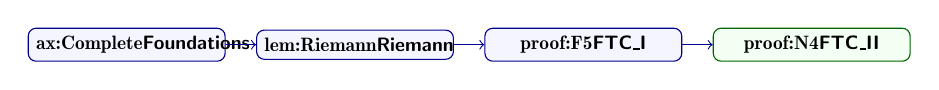
\begin{tikzpicture}
\tikzstyle{dep}=[draw=blue!55!black,fill=blue!4,rounded corners=1mm,
 text width=23mm,text centered,inner sep=1mm]
\tikzstyle{done}=[dep,draw=green!40!black,fill=green!5]
\tikzstyle{flow}=[->,blue!55!black]
\node[dep] (a) at (0.0,0) {\scriptsize \hyperlink{ax:Complete}{\textsf{Foundations}}};
\node[dep] (w) at (2.9,0) {\scriptsize \hyperlink{lem:Riemann}{\textsf{Riemann}}};
\node[dep] (p) at (5.8,0) {\scriptsize \hyperlink{proof:F5}{\textsf{FTC\_I}}};
\node[done] (m) at (8.7,0) {\scriptsize \hyperlink{proof:N4}{\textsf{FTC\_II}}};
\draw[flow] (a)--(w);
\draw[flow] (w)--(p);
\draw[flow] (p)--(m);
\end{tikzpicture}

\par\vspace{3mm}
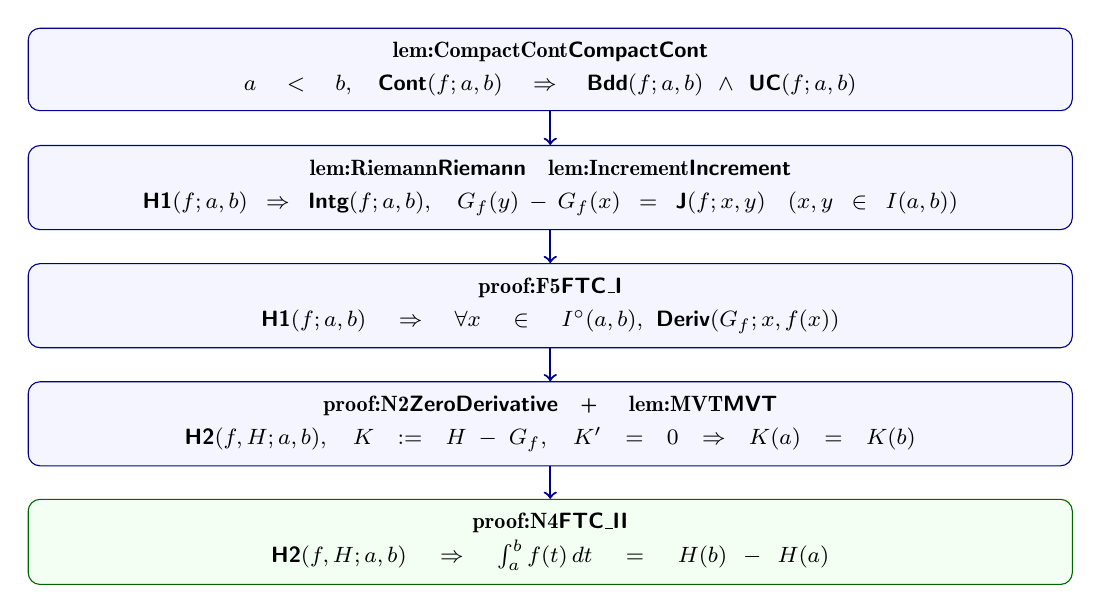
\begin{tikzpicture}
\tikzstyle{dep}=[draw=blue!55!black,fill=blue!4,rounded corners=1.5mm,
 text width=12.9cm,text centered,inner sep=1.8mm]
\tikzstyle{done}=[dep,draw=green!40!black,fill=green!5]
\tikzstyle{flow}=[->,thick,blue!55!black]
\node[dep] (ap) at (0,-0.0) {\footnotesize
\hyperlink{lem:CompactCont}{\textsf{CompactCont}}\\
$a<b,\quad\textsf{Cont}(f;a,b)\Rightarrow
\textsf{Bdd}(f;a,b)\land\textsf{UC}(f;a,b)$};
\node[dep] (win) at (0,-1.5) {\footnotesize
\hyperlink{lem:Riemann}{\textsf{Riemann}}\quad
\hyperlink{lem:Increment}{\textsf{Increment}}\\
$\textsf{H1}(f;a,b)\Rightarrow\textsf{Intg}(f;a,b),\quad
G_f(y)-G_f(x)=\textsf{J}(f;x,y)\quad(x,y\in I(a,b))$};
\node[dep] (seq) at (0,-3.0) {\footnotesize
\hyperlink{proof:F5}{\textsf{FTC\_I}}\\
$\textsf{H1}(f;a,b)\Rightarrow
\forall x\in I^\circ(a,b),\ \textsf{Deriv}(G_f;x,f(x))$};
\node[dep] (code) at (0,-4.5) {\footnotesize
\hyperlink{proof:N2}{\textsf{ZeroDerivative}}\quad+
\quad\hyperlink{lem:MVT}{\textsf{MVT}}\\
$\textsf{H2}(f,H;a,b),\quad K:=H-G_f,\quad
K'=0\Rightarrow K(a)=K(b)$};
\node[done] (result) at (0,-6.0) {\footnotesize
\hyperlink{proof:N4}{\textsf{FTC\_II}}\\
$\textsf{H2}(f,H;a,b)\Rightarrow\int_a^b f(t)\,dt=H(b)-H(a)$};
\draw[flow] (ap)--(win);
\draw[flow] (win)--(seq);
\draw[flow] (seq)--(code);
\draw[flow] (code)--(result);
\end{tikzpicture}
\par
\end{minipage}}
\end{figure}

\clearpage
\setstretch{1.2}\pagestyle{plain}\pagenumbering{arabic} %
\hypersetup{pageanchor=true}

\section*{Scope and contribution}

\begin{center}
{\small $\mathsf{ContinuousRiemannFTC}_{\mathrm{I},\mathrm{II}},\quad 
\mathsf{H1}(f;a,b)\Longleftrightarrow a<b\wedge \mathsf{Cont}(f;a,b).$}

{\small $\mathsf{RealCompleteness}\Rightarrow \mathsf{CompactCont}%
\Rightarrow \mathsf{Riemann}\Rightarrow \mathsf{FTC\_I}.$}

{\small $\mathsf{FTC\_I}\wedge \mathsf{MVT}\Rightarrow \mathsf{FTC\_II}.$}

{\small $\mathsf{TypedMathematicalExposition}\neq \mathsf{ExecutableLean}.$}
\end{center}

{\scriptsize \setlength{\parskip}{0pt}\nointerlineskip
\noindent 
\begin{tabular}{|@{}>{\centering\arraybackslash}m{\FTCOneColumnBody}|}
\hline
\hypertarget{theorem:FTC}{$\displaystyle \mathsf{FTC}:\ \forall(a,b:\mathsf{%
Real})\ (f,H:\mathsf{RF}),\ \allowbreak\mathsf{H1}(f;a,b)\Rightarrow%
\allowbreak\mathsf{Intg}(f;a,b)\land\mathsf{Cont}(G_f;a,b)\land\allowbreak(%
\forall x:\mathsf{Real},\ a<x<b\Rightarrow\mathsf{Deriv}(G_f;x,f(x)))\land%
\allowbreak(\mathsf{H2}(f,H;a,b)\Rightarrow\mathsf{J}(f;a,b)=H(b)-H(a))$} \\ 
\hline
\end{tabular}%
}

{\scriptsize \setlength{\parskip}{0pt}\nointerlineskip
\noindent 
\begin{tabular}{|@{}>{\centering\arraybackslash}m{\FTCOneColumnBody}|}
\hline
$\displaystyle \mathsf{Context\_0}:=$\par$\displaystyle a,b:\mathsf{Real}%
,\quad\mathsf{RF}:=\mathsf{Real}\to\mathsf{Real},$\par$\displaystyle f,H:%
\mathsf{RF},\quad G_f:=\lambda x,\ \mathsf{J}(f;a,x).$ \\ \hline
\end{tabular}%
}

\section{\protect\scriptsize Foundations}

{\scriptsize {\ }}

{\scriptsize \setlength{\parskip}{0pt}\nointerlineskip
\noindent 
\begin{tabular}{|@{}>{\centering\arraybackslash}m{\FTCOneColumnBody}|}
\hline
$\displaystyle \mathsf{Foundations}$ \\ \hline
\end{tabular}%
}

{\scriptsize \setlength{\parskip}{0pt}\nointerlineskip
\noindent 
\begin{tabular}{|@{}>{\centering\arraybackslash}m{0.19251\linewidth}|>{\centering\arraybackslash}m{0.16845\linewidth}|>{\centering\arraybackslash}m{0.53904\linewidth}|}
\hline
$\displaystyle \mathsf{Id}$ & $\displaystyle \mathsf{Kind}$ & $\displaystyle 
\mathsf{Formula}$ \\ \hline
\end{tabular}%
}

{\scriptsize \setlength{\parskip}{0pt}\nointerlineskip
\noindent 
\begin{tabular}{|@{}>{\centering\arraybackslash}m{0.19251\linewidth}|>{\centering\arraybackslash}m{0.16845\linewidth}|>{\centering\arraybackslash}m{0.53904\linewidth}|}
\hline
\hypertarget{ax:Real}{$\displaystyle \mathsf{Real}$} & $\displaystyle 
\mathsf{axiom}$ & $\displaystyle \mathsf{LinearOrderedField}(\mathsf{Real}),$%
\par$\displaystyle \mathsf{Archimedean}(\mathsf{Real}),$\par$\displaystyle %
\forall c:\mathsf{Real},\ \exists n:\mathsf{Nat},\ c<n.$ \\ \hline
\end{tabular}%
}

{\scriptsize \setlength{\parskip}{0pt}\nointerlineskip
\noindent 
\begin{tabular}{|@{}>{\centering\arraybackslash}m{0.19251\linewidth}|>{\centering\arraybackslash}m{0.16845\linewidth}|>{\centering\arraybackslash}m{0.53904\linewidth}|}
\hline
\hypertarget{ax:Complete}{$\displaystyle \mathsf{Complete}$} & $%
\displaystyle \mathsf{axiom}$ & $\displaystyle \mathsf{sSup}:\mathsf{Set}(%
\mathsf{Real})\to\mathsf{Real},$\par$\displaystyle \mathsf{BA}%
(S):\Longleftrightarrow\exists M,\ \forall s\in S,\ s\le M,$\par$%
\displaystyle S\ne\varnothing\land\mathsf{BA}(S)\Rightarrow$\par$%
\displaystyle (\forall s\in S,\ s\le\mathsf{sSup}(S))$\par$\displaystyle %
\land(\forall U,\ (\forall s\in S,\ s\le U)\Rightarrow\mathsf{sSup}(S)\le
U), $\par$\displaystyle \neg(S\ne\varnothing\land\mathsf{BA}(S))\Rightarrow%
\mathsf{sSup}(S)=0,$\par$\displaystyle \sup S:=\mathsf{sSup}(S),\quad\inf
S:=-\mathsf{sSup}(\{-s\mid s\in S\}).$ \\ \hline
\end{tabular}%
}

{\scriptsize \setlength{\parskip}{0pt}\nointerlineskip
\noindent 
\begin{tabular}{|@{}>{\centering\arraybackslash}m{0.19251\linewidth}|>{\centering\arraybackslash}m{0.16845\linewidth}|>{\centering\arraybackslash}m{0.53904\linewidth}|}
\hline
\hypertarget{ax:Nat}{$\displaystyle \mathsf{Nat}$} & $\displaystyle \mathsf{%
axiom}$ & $\displaystyle \mathsf{Induction}(\mathsf{Nat})\land\mathsf{%
Recursion}(\mathsf{Nat}),$\par$\displaystyle (\exists n:\mathsf{Nat},\
P(n))\Rightarrow$\par$\displaystyle \exists n,\ P(n)\land\forall j<n,\ \neg
P(j),$\par$\displaystyle \mathsf{Fin}(n):=\{i:\mathsf{Nat}\mid i<n\}.$ \\ 
\hline
\end{tabular}%
}

{\scriptsize \setlength{\parskip}{0pt}\nointerlineskip
\noindent 
\begin{tabular}{|@{}>{\centering\arraybackslash}m{0.19251\linewidth}|>{\centering\arraybackslash}m{0.16845\linewidth}|>{\centering\arraybackslash}m{0.53904\linewidth}|}
\hline
\hypertarget{ax:Classical}{$\displaystyle \mathsf{Classical}$} & $%
\displaystyle \mathsf{axiom}$ & $\displaystyle \forall P:\mathsf{Prop},\
P\lor\neg P,$\par$\displaystyle P:\mathsf{Nat}\to\mathsf{Real}\to\mathsf{Prop%
},$\par$\displaystyle (\forall n,\ \exists x,\ P(n,x))\Rightarrow$\par$%
\displaystyle \exists u:\mathsf{Nat}\to\mathsf{Real},\ \forall n,\ P(n,u_n).$
\\ \hline
\end{tabular}%
}

{\scriptsize \ }

\section{\protect\scriptsize Definitions}

{\scriptsize {\ }}

{\scriptsize \setlength{\parskip}{0pt}\nointerlineskip
\noindent 
\begin{tabular}{|@{}>{\centering\arraybackslash}m{\FTCOneColumnBody}|}
\hline
$\displaystyle \mathsf{Definitions}$ \\ \hline
\end{tabular}%
}

{\scriptsize \setlength{\parskip}{0pt}\nointerlineskip
\noindent 
\begin{tabular}{|@{}>{\centering\arraybackslash}m{0.19251\linewidth}|>{\centering\arraybackslash}m{0.16845\linewidth}|>{\centering\arraybackslash}m{0.53904\linewidth}|}
\hline
$\displaystyle \mathsf{Id}$ & $\displaystyle \mathsf{Kind}$ & $\displaystyle 
\mathsf{Formula}$ \\ \hline
\end{tabular}%
}

{\scriptsize \setlength{\parskip}{0pt}\nointerlineskip
\noindent 
\begin{tabular}{|@{}>{\centering\arraybackslash}m{0.19251\linewidth}|>{\centering\arraybackslash}m{0.16845\linewidth}|>{\centering\arraybackslash}m{0.53904\linewidth}|}
\hline
\hypertarget{def:Intervals}{$\displaystyle \mathsf{Intervals}$} & $%
\displaystyle \mathsf{def}$ & $\displaystyle I(r,s):=\{x:\mathsf{Real}\mid
r\le x\le s\},$\par$\displaystyle I^\circ(r,s):=\{x:\mathsf{Real}\mid
r<x<s\},$\par$\displaystyle \mathsf{PosNat}:=\{n:\mathsf{Nat}\mid0<n\}.$ \\ 
\hline
\end{tabular}%
}

{\scriptsize \setlength{\parskip}{0pt}\nointerlineskip
\noindent 
\begin{tabular}{|@{}>{\centering\arraybackslash}m{0.19251\linewidth}|>{\centering\arraybackslash}m{0.16845\linewidth}|>{\centering\arraybackslash}m{0.53904\linewidth}|}
\hline
\hypertarget{def:Conv}{$\displaystyle \mathsf{Conv}$} & $\displaystyle 
\mathsf{def}$ & $\displaystyle u:\mathsf{Nat}\to\mathsf{Real},\quad\xi:%
\mathsf{Real},$\par$\displaystyle \mathsf{Conv}(u,\xi):\Longleftrightarrow$%
\par$\displaystyle \forall\varepsilon:\mathsf{Real},\
\varepsilon>0\Rightarrow$\par$\displaystyle \exists N:\mathsf{Nat},\ \forall
n\ge N,\ |u_n-\xi|<\varepsilon.$ \\ \hline
\end{tabular}%
}

{\scriptsize \setlength{\parskip}{0pt}\nointerlineskip
\noindent 
\begin{tabular}{|@{}>{\centering\arraybackslash}m{0.19251\linewidth}|>{\centering\arraybackslash}m{0.16845\linewidth}|>{\centering\arraybackslash}m{0.53904\linewidth}|}
\hline
\hypertarget{def:Cont}{$\displaystyle \mathsf{Cont}$} & $\displaystyle 
\mathsf{def}$ & $\displaystyle \mathsf{Cont}(f;r,s):\Longleftrightarrow$\par$%
\displaystyle \forall x\in I(r,s),\ \forall\varepsilon>0,\ \exists\delta>0,$%
\par$\displaystyle \forall t\in I(r,s),$\par$\displaystyle %
|t-x|<\delta\Rightarrow|f(t)-f(x)|<\varepsilon.$ \\ \hline
\end{tabular}%
}

{\scriptsize \setlength{\parskip}{0pt}\nointerlineskip
\noindent 
\begin{tabular}{|@{}>{\centering\arraybackslash}m{0.19251\linewidth}|>{\centering\arraybackslash}m{0.16845\linewidth}|>{\centering\arraybackslash}m{0.53904\linewidth}|}
\hline
\hypertarget{def:Uniform}{$\displaystyle \mathsf{Uniform}$} & $\displaystyle 
\mathsf{def}$ & $\displaystyle \mathsf{UC}(f;r,s):\Longleftrightarrow$\par$%
\displaystyle \forall\varepsilon>0,\ \exists\delta>0,\ \forall x,t\in
I(r,s), $\par$\displaystyle |t-x|<\delta\Rightarrow|f(t)-f(x)|<\varepsilon.$
\\ \hline
\end{tabular}%
}

{\scriptsize \setlength{\parskip}{0pt}\nointerlineskip
\noindent 
\begin{tabular}{|@{}>{\centering\arraybackslash}m{0.19251\linewidth}|>{\centering\arraybackslash}m{0.16845\linewidth}|>{\centering\arraybackslash}m{0.53904\linewidth}|}
\hline
\hypertarget{def:Bdd}{$\displaystyle \mathsf{Bdd}$} & $\displaystyle \mathsf{%
def}$ & $\displaystyle \mathsf{Bdd}(f;r,s):\Longleftrightarrow$\par$%
\displaystyle \exists M:\mathsf{Real},\ M\ge0$\par$\displaystyle %
\land\forall x\in I(r,s),\ |f(x)|\le M.$ \\ \hline
\end{tabular}%
}

{\scriptsize \setlength{\parskip}{0pt}\nointerlineskip
\noindent 
\begin{tabular}{|@{}>{\centering\arraybackslash}m{0.19251\linewidth}|>{\centering\arraybackslash}m{0.16845\linewidth}|>{\centering\arraybackslash}m{0.53904\linewidth}|}
\hline
\hypertarget{def:InfHits}{$\displaystyle \mathsf{InfHits}$} & $\displaystyle 
\mathsf{def}$ & $\displaystyle u:\mathsf{Nat}\to\mathsf{Real},$\par$%
\displaystyle \mathsf{IH}(u;r,s):\Longleftrightarrow$\par$\displaystyle %
\forall N:\mathsf{Nat},\ \exists n\ge N,\ u_n\in I(r,s).$ \\ \hline
\end{tabular}%
}

{\scriptsize \setlength{\parskip}{0pt}\nointerlineskip
\noindent 
\begin{tabular}{|@{}>{\centering\arraybackslash}m{0.19251\linewidth}|>{\centering\arraybackslash}m{0.16845\linewidth}|>{\centering\arraybackslash}m{0.53904\linewidth}|}
\hline
\hypertarget{def:Deriv}{$\displaystyle \mathsf{Deriv}$} & $\displaystyle 
\mathsf{def}$ & $\displaystyle \mathsf{Deriv}(H;x,d):\Longleftrightarrow$\par%
$\displaystyle \forall\varepsilon>0,\ \exists\delta>0,\ \forall h:\mathsf{%
Real},$\par$\displaystyle 0<|h|<\delta\Rightarrow$\par$\displaystyle \left|%
\frac{H(x+h)-H(x)}h-d\right|<\varepsilon,$\par$\displaystyle \mathsf{Diff}%
(H;r,s):\Longleftrightarrow$\par$\displaystyle \forall x\in I^\circ(r,s),\
\exists d,\ \mathsf{Deriv}(H;x,d).$ \\ \hline
\end{tabular}%
}

{\scriptsize \setlength{\parskip}{0pt}\nointerlineskip
\noindent 
\begin{tabular}{|@{}>{\centering\arraybackslash}m{0.19251\linewidth}|>{\centering\arraybackslash}m{0.16845\linewidth}|>{\centering\arraybackslash}m{0.53904\linewidth}|}
\hline
\hypertarget{def:Lists}{$\displaystyle \mathsf{Lists}$} & $\displaystyle 
\mathsf{def}$ & $\displaystyle \mathsf{List}(T):=\mathsf{Sigma}(\lambda n:%
\mathsf{Nat},\ \mathsf{Fin}(n)\to T),$\par$\displaystyle \mathsf{StrictSorted%
}(L):\Longleftrightarrow$\par$\displaystyle \forall i<j<|L|,\ L_i<L_j,$\par$%
\displaystyle |L\mathbin{+\!\!+}Q|:=|L|+|Q|,$\par$\displaystyle (L%
\mathbin{+\!\!+}Q)_i:=\mathsf{if}\ i<|L|\ \mathsf{then}\ L_i$\par$%
\displaystyle \mathsf{else}\ Q_{i-|L|},\quad\mathsf{tail}(z::L):=L.$ \\ 
\hline
\end{tabular}%
}

{\scriptsize \setlength{\parskip}{0pt}\nointerlineskip
\noindent 
\begin{tabular}{|@{}>{\centering\arraybackslash}m{0.19251\linewidth}|>{\centering\arraybackslash}m{0.16845\linewidth}|>{\centering\arraybackslash}m{0.53904\linewidth}|}
\hline
\hypertarget{def:Part}{$\displaystyle \mathsf{Part}$} & $\displaystyle 
\mathsf{def}$ & $\displaystyle P=(m,x),\quad m:\mathsf{PosNat},$\par$%
\displaystyle x:\mathsf{Fin}(m+1)\to\mathsf{Real},$\par$\displaystyle P:%
\mathsf{Part}(r,s):\Longleftrightarrow$\par$\displaystyle x_0=r\land
x_m=s\land\forall i<m,\ x_i<x_{i+1},$\par$\displaystyle \Delta
P_i:=x_{i+1}-x_i,\quad\mathsf{nodes}(P):=[x_0,\ldots,x_m],$\par$%
\displaystyle P\preceq Q:\Longleftrightarrow\forall i\le m_P,\ \exists j\le
m_Q,\ x_i=y_j.$ \\ \hline
\end{tabular}%
}

{\scriptsize \setlength{\parskip}{0pt}\nointerlineskip
\noindent 
\begin{tabular}{|@{}>{\centering\arraybackslash}m{0.19251\linewidth}|>{\centering\arraybackslash}m{0.16845\linewidth}|>{\centering\arraybackslash}m{0.53904\linewidth}|}
\hline
\hypertarget{def:Darboux}{$\displaystyle \mathsf{Darboux}$} & $\displaystyle 
\mathsf{def}$ & $\displaystyle \ell_i(f,P):=\inf\{f(t)\mid t\in
I(x_i,x_{i+1})\},$\par$\displaystyle u_i(f,P):=\sup\{f(t)\mid t\in
I(x_i,x_{i+1})\},$\par$\displaystyle \mathsf{L}(f,P):=\sum_{i<m_P}%
\ell_i(f,P)\Delta P_i,$\par$\displaystyle \mathsf{U}(f,P):=%
\sum_{i<m_P}u_i(f,P)\Delta P_i,$\par$\displaystyle D^-(f;r,s):=\sup_{P:%
\mathsf{Part}(r,s)}\mathsf{L}(f,P),$\par$\displaystyle D^+(f;r,s):=\inf_{P:%
\mathsf{Part}(r,s)}\mathsf{U}(f,P).$ \\ \hline
\end{tabular}%
}

{\scriptsize \setlength{\parskip}{0pt}\nointerlineskip
\noindent 
\begin{tabular}{|@{}>{\centering\arraybackslash}m{0.19251\linewidth}|>{\centering\arraybackslash}m{0.16845\linewidth}|>{\centering\arraybackslash}m{0.53904\linewidth}|}
\hline
\hypertarget{def:Integral}{$\displaystyle \mathsf{Integral}$} & $%
\displaystyle \mathsf{def}$ & $\displaystyle \alpha:=\min(r,s),\quad\beta:=%
\max(r,s),$\par$\displaystyle \mathsf{Intg}(f;r,s):\Longleftrightarrow r=s\
\lor$\par$\displaystyle (\mathsf{Bdd}(f;\alpha,\beta)\land
D^-(f;\alpha,\beta)=D^+(f;\alpha,\beta)),$\par$\displaystyle \mathsf{J}%
(f;r,s):=\mathsf{if}\ r=s\ \mathsf{then}\ 0$\par$\displaystyle \mathsf{else\
if}\ \neg\mathsf{Intg}(f;r,s)\ \mathsf{then}\ 0$\par$\displaystyle \mathsf{%
else\ if}\ r<s\ \mathsf{then}\ D^-(f;r,s)$\par$\displaystyle \mathsf{else}\
-D^-(f;s,r),$\par$\displaystyle \int_r^s f(t)\,dt:=\mathsf{J}(f;r,s).$ \\ 
\hline
\end{tabular}%
}

{\scriptsize \setlength{\parskip}{0pt}\nointerlineskip
\noindent 
\begin{tabular}{|@{}>{\centering\arraybackslash}m{0.19251\linewidth}|>{\centering\arraybackslash}m{0.16845\linewidth}|>{\centering\arraybackslash}m{0.53904\linewidth}|}
\hline
\hypertarget{def:Hyp}{$\displaystyle \mathsf{Hyp}$} & $\displaystyle \mathsf{%
def}$ & $\displaystyle \mathsf{H1}(f;a,b):\Longleftrightarrow a<b\land%
\mathsf{Cont}(f;a,b),$\par$\displaystyle \mathsf{H2}(f,H;a,b):%
\Longleftrightarrow$\par$\displaystyle \mathsf{H1}(f;a,b)\land\mathsf{Cont}%
(H;a,b)$\par$\displaystyle \land\forall x\in I^\circ(a,b),\ \mathsf{Deriv}%
(H;x,f(x)),$\par$\displaystyle G_f:=\lambda x:\mathsf{Real},\ \mathsf{J}%
(f;a,x).$ \\ \hline
\end{tabular}%
}

{\scriptsize \ }

\section{\protect\scriptsize Logical Rules}

{\scriptsize {\ }}

{\scriptsize \setlength{\parskip}{0pt}\nointerlineskip
\noindent 
\begin{tabular}{|@{}>{\centering\arraybackslash}m{\FTCOneColumnBody}|}
\hline
$\displaystyle \mathsf{Logic}$ \\ \hline
\end{tabular}%
}

{\scriptsize \setlength{\parskip}{0pt}\nointerlineskip
\noindent 
\begin{tabular}{|@{}>{\centering\arraybackslash}m{0.19251\linewidth}|>{\centering\arraybackslash}m{0.16845\linewidth}|>{\centering\arraybackslash}m{0.53904\linewidth}|}
\hline
$\displaystyle \mathsf{Id}$ & $\displaystyle \mathsf{Symbol}$ & $%
\displaystyle \mathsf{Formula}$ \\ \hline
\end{tabular}%
}

{\scriptsize \setlength{\parskip}{0pt}\nointerlineskip
\noindent 
\begin{tabular}{|@{}>{\centering\arraybackslash}m{0.19251\linewidth}|>{\centering\arraybackslash}m{0.16845\linewidth}|>{\centering\arraybackslash}m{0.53904\linewidth}|}
\hline
\hypertarget{rule:AllI}{$\displaystyle \mathsf{AllI}$} & $\displaystyle %
\forall I$ & \rule[-3.3ex]{0pt}{7.8ex}$\displaystyle \dfrac{\Gamma\vdash
P(x)\quad x\notin\mathsf{FV}(\Gamma)}{\Gamma\vdash\forall x\,P(x)}$ \\ \hline
\end{tabular}%
}

{\scriptsize \setlength{\parskip}{0pt}\nointerlineskip
\noindent 
\begin{tabular}{|@{}>{\centering\arraybackslash}m{0.19251\linewidth}|>{\centering\arraybackslash}m{0.16845\linewidth}|>{\centering\arraybackslash}m{0.53904\linewidth}|}
\hline
\hypertarget{rule:AllE}{$\displaystyle \mathsf{AllE}$} & $\displaystyle %
\forall E$ & \rule[-3.3ex]{0pt}{7.8ex}$\displaystyle \dfrac{%
\Gamma\vdash\forall x\,P(x)}{\Gamma\vdash P(a)}$ \\ \hline
\end{tabular}%
}

{\scriptsize \setlength{\parskip}{0pt}\nointerlineskip
\noindent 
\begin{tabular}{|@{}>{\centering\arraybackslash}m{0.19251\linewidth}|>{\centering\arraybackslash}m{0.16845\linewidth}|>{\centering\arraybackslash}m{0.53904\linewidth}|}
\hline
\hypertarget{rule:AndI}{$\displaystyle \mathsf{AndI}$} & $\displaystyle %
\wedge I$ & \rule[-3.3ex]{0pt}{7.8ex}$\displaystyle \dfrac{\Gamma\vdash
P\quad\Gamma\vdash Q}{\Gamma\vdash P\land Q}$ \\ \hline
\end{tabular}%
}

{\scriptsize \setlength{\parskip}{0pt}\nointerlineskip
\noindent 
\begin{tabular}{|@{}>{\centering\arraybackslash}m{0.19251\linewidth}|>{\centering\arraybackslash}m{0.16845\linewidth}|>{\centering\arraybackslash}m{0.53904\linewidth}|}
\hline
\hypertarget{rule:AndE}{$\displaystyle \mathsf{AndE}$} & $\displaystyle %
\wedge E$ & \rule[-3.3ex]{0pt}{7.8ex}$\displaystyle \dfrac{\Gamma\vdash
P\land Q}{\Gamma\vdash P}\quad\dfrac{\Gamma\vdash P\land Q}{\Gamma\vdash Q}$
\\ \hline
\end{tabular}%
}

{\scriptsize \setlength{\parskip}{0pt}\nointerlineskip
\noindent 
\begin{tabular}{|@{}>{\centering\arraybackslash}m{0.19251\linewidth}|>{\centering\arraybackslash}m{0.16845\linewidth}|>{\centering\arraybackslash}m{0.53904\linewidth}|}
\hline
\hypertarget{rule:ImpI}{$\displaystyle \mathsf{ImpI}$} & $\displaystyle \to
I $ & \rule[-3.3ex]{0pt}{7.8ex}$\displaystyle \dfrac{\Gamma,P\vdash Q}{%
\Gamma\vdash P\to Q}$ \\ \hline
\end{tabular}%
}

{\scriptsize \setlength{\parskip}{0pt}\nointerlineskip
\noindent 
\begin{tabular}{|@{}>{\centering\arraybackslash}m{0.19251\linewidth}|>{\centering\arraybackslash}m{0.16845\linewidth}|>{\centering\arraybackslash}m{0.53904\linewidth}|}
\hline
\hypertarget{rule:MP}{$\displaystyle \mathsf{MP}$} & $\displaystyle \to E$ & 
\rule[-3.3ex]{0pt}{7.8ex}$\displaystyle \dfrac{\Gamma\vdash
P\quad\Gamma\vdash P\to Q}{\Gamma\vdash Q}$ \\ \hline
\end{tabular}%
}

{\scriptsize \setlength{\parskip}{0pt}\nointerlineskip
\noindent 
\begin{tabular}{|@{}>{\centering\arraybackslash}m{0.19251\linewidth}|>{\centering\arraybackslash}m{0.16845\linewidth}|>{\centering\arraybackslash}m{0.53904\linewidth}|}
\hline
\hypertarget{rule:ExistsI}{$\displaystyle \mathsf{ExistsI}$} & $%
\displaystyle \exists I$ & \rule[-3.3ex]{0pt}{7.8ex}$\displaystyle \dfrac{%
\Gamma\vdash P(a)}{\Gamma\vdash\exists x\,P(x)}$ \\ \hline
\end{tabular}%
}

{\scriptsize \setlength{\parskip}{0pt}\nointerlineskip
\noindent 
\begin{tabular}{|@{}>{\centering\arraybackslash}m{0.19251\linewidth}|>{\centering\arraybackslash}m{0.16845\linewidth}|>{\centering\arraybackslash}m{0.53904\linewidth}|}
\hline
\hypertarget{rule:ExistsE}{$\displaystyle \mathsf{ExistsE}$} & $%
\displaystyle \exists E$ & \rule[-3.3ex]{0pt}{7.8ex}$\displaystyle \dfrac{%
\Gamma\vdash\exists xP(x)\quad\Gamma,P(y)\vdash Q}{\Gamma\vdash Q}$\par$%
\displaystyle y\notin\mathsf{FV}(\Gamma,Q).$ \\ \hline
\end{tabular}%
}

{\scriptsize \setlength{\parskip}{0pt}\nointerlineskip
\noindent 
\begin{tabular}{|@{}>{\centering\arraybackslash}m{0.19251\linewidth}|>{\centering\arraybackslash}m{0.16845\linewidth}|>{\centering\arraybackslash}m{0.53904\linewidth}|}
\hline
\hypertarget{rule:Eq}{$\displaystyle \mathsf{Eq}$} & $\displaystyle =E$ & 
\rule[-3.3ex]{0pt}{7.8ex}$\displaystyle \dfrac{\Gamma\vdash
a=b\quad\Gamma\vdash P(a)}{\Gamma\vdash P(b)}$ \\ \hline
\end{tabular}%
}

{\scriptsize \setlength{\parskip}{0pt}\nointerlineskip
\noindent 
\begin{tabular}{|@{}>{\centering\arraybackslash}m{0.19251\linewidth}|>{\centering\arraybackslash}m{0.16845\linewidth}|>{\centering\arraybackslash}m{0.53904\linewidth}|}
\hline
\hypertarget{rule:Cases}{$\displaystyle \mathsf{Cases}$} & $\displaystyle %
\vee E$ & \rule[-3.3ex]{0pt}{7.8ex}$\displaystyle \dfrac{\Gamma\vdash P\lor
Q\quad\Gamma,P\vdash R\quad\Gamma,Q\vdash R}{\Gamma\vdash R}$ \\ \hline
\end{tabular}%
}

{\scriptsize \setlength{\parskip}{0pt}\nointerlineskip
\noindent 
\begin{tabular}{|@{}>{\centering\arraybackslash}m{0.19251\linewidth}|>{\centering\arraybackslash}m{0.16845\linewidth}|>{\centering\arraybackslash}m{0.53904\linewidth}|}
\hline
\hypertarget{rule:NotI}{$\displaystyle \mathsf{NotI}$} & $\displaystyle \neg
I$ & \rule[-3.3ex]{0pt}{7.8ex}$\displaystyle \dfrac{\Gamma,P\vdash\bot}{%
\Gamma\vdash\neg P}$ \\ \hline
\end{tabular}%
}

{\scriptsize \setlength{\parskip}{0pt}\nointerlineskip
\noindent 
\begin{tabular}{|@{}>{\centering\arraybackslash}m{0.19251\linewidth}|>{\centering\arraybackslash}m{0.16845\linewidth}|>{\centering\arraybackslash}m{0.53904\linewidth}|}
\hline
\hypertarget{rule:FalseE}{$\displaystyle \mathsf{FalseE}$} & $\displaystyle %
\bot E$ & \rule[-3.3ex]{0pt}{7.8ex}$\displaystyle \dfrac{\Gamma\vdash\bot}{%
\Gamma\vdash P}$ \\ \hline
\end{tabular}%
}

{\scriptsize \setlength{\parskip}{0pt}\nointerlineskip
\noindent 
\begin{tabular}{|@{}>{\centering\arraybackslash}m{0.19251\linewidth}|>{\centering\arraybackslash}m{0.16845\linewidth}|>{\centering\arraybackslash}m{0.53904\linewidth}|}
\hline
\hypertarget{rule:Classical}{$\displaystyle \mathsf{Classical}$} & $%
\displaystyle \neg\neg E$ & \rule[-3.3ex]{0pt}{7.8ex}$\displaystyle \dfrac{%
\Gamma\vdash\neg\neg P}{\Gamma\vdash P}$ \\ \hline
\end{tabular}%
}

{\scriptsize \ }

\section{\protect\scriptsize Lemmas and Theorems}

{\scriptsize {\ }}

{\scriptsize \setlength{\parskip}{0pt}\nointerlineskip
\noindent 
\begin{tabular}{|@{}>{\centering\arraybackslash}m{\FTCOneColumnBody}|}
\hline
$\displaystyle \mathsf{Lemmas}$ \\ \hline
\end{tabular}%
}

{\scriptsize \setlength{\parskip}{0pt}\nointerlineskip
\noindent 
\begin{tabular}{|@{}>{\centering\arraybackslash}m{0.19251\linewidth}|>{\centering\arraybackslash}m{0.16845\linewidth}|>{\centering\arraybackslash}m{0.53904\linewidth}|}
\hline
$\displaystyle \mathsf{Id}$ & $\displaystyle \mathsf{Proof}$ & $%
\displaystyle \mathsf{Formula}$ \\ \hline
\end{tabular}%
}

{\scriptsize \setlength{\parskip}{0pt}\nointerlineskip
\noindent 
\begin{tabular}{|@{}>{\centering\arraybackslash}m{0.19251\linewidth}|>{\centering\arraybackslash}m{0.16845\linewidth}|>{\centering\arraybackslash}m{0.53904\linewidth}|}
\hline
\hypertarget{lem:Subsequence}{$\displaystyle \mathsf{Subsequence}$} & 
\hyperlink{proof:K5}{$\displaystyle \mathsf{K5}$} & $\displaystyle a\le
b,\quad\forall n,\ u_n\in I(a,b)\Rightarrow$\par$\displaystyle \exists\xi\in
I(a,b),\ \exists\nu:\mathsf{Nat}\to\mathsf{Nat},$\par$\displaystyle (\forall
k,\ \nu_{k+1}>\nu_k)\land\mathsf{Conv}(u\circ\nu,\xi).$ \\ \hline
\end{tabular}%
}

{\scriptsize \setlength{\parskip}{0pt}\nointerlineskip
\noindent 
\begin{tabular}{|@{}>{\centering\arraybackslash}m{0.19251\linewidth}|>{\centering\arraybackslash}m{0.16845\linewidth}|>{\centering\arraybackslash}m{0.53904\linewidth}|}
\hline
\hypertarget{lem:CompactCont}{$\displaystyle \mathsf{CompactCont}$} & 
\hyperlink{proof:C7}{$\displaystyle \mathsf{C7}$} & $\displaystyle a\le
b\land\mathsf{Cont}(f;a,b)\Rightarrow$\par$\displaystyle \mathsf{Bdd}%
(f;a,b)\land\mathsf{UC}(f;a,b),$\par$\displaystyle \exists p,q\in I(a,b),\
\forall x\in I(a,b),\ f(p)\le f(x)\le f(q).$ \\ \hline
\end{tabular}%
}

{\scriptsize \setlength{\parskip}{0pt}\nointerlineskip
\noindent 
\begin{tabular}{|@{}>{\centering\arraybackslash}m{0.19251\linewidth}|>{\centering\arraybackslash}m{0.16845\linewidth}|>{\centering\arraybackslash}m{0.53904\linewidth}|}
\hline
\hypertarget{lem:Riemann}{$\displaystyle \mathsf{Riemann}$} & \hyperlink{proof:P9}%
{$\displaystyle \mathsf{P9}$} & $\displaystyle \mathsf{H1}(f;a,b)\Rightarrow$%
\par$\displaystyle \forall r,s\in I(a,b),\ \mathsf{Intg}(f;r,s).$ \\ \hline
\end{tabular}%
}

{\scriptsize \setlength{\parskip}{0pt}\nointerlineskip
\noindent 
\begin{tabular}{|@{}>{\centering\arraybackslash}m{0.19251\linewidth}|>{\centering\arraybackslash}m{0.16845\linewidth}|>{\centering\arraybackslash}m{0.53904\linewidth}|}
\hline
\hypertarget{lem:Increment}{$\displaystyle \mathsf{Increment}$} & \hyperlink{proof:E6}%
{$\displaystyle \mathsf{E6}$} & $\displaystyle \mathsf{H1}(f;a,b)\Rightarrow$%
\par$\displaystyle \forall x,y\in I(a,b),$\par$\displaystyle G_f(y)-G_f(x)=%
\mathsf{J}(f;x,y).$ \\ \hline
\end{tabular}%
}

{\scriptsize \setlength{\parskip}{0pt}\nointerlineskip
\noindent 
\begin{tabular}{|@{}>{\centering\arraybackslash}m{0.19251\linewidth}|>{\centering\arraybackslash}m{0.16845\linewidth}|>{\centering\arraybackslash}m{0.53904\linewidth}|}
\hline
\hypertarget{lem:Rolle}{$\displaystyle \mathsf{Rolle}$} & \hyperlink{proof:R4}%
{$\displaystyle \mathsf{R4}$} & $\displaystyle a<b\land\mathsf{Cont}%
(H;a,b)\land\mathsf{Diff}(H;a,b)$\par$\displaystyle \land
H(a)=H(b)\Rightarrow$\par$\displaystyle \exists c\in I^\circ(a,b),\ \mathsf{%
Deriv}(H;c,0).$ \\ \hline
\end{tabular}%
}

{\scriptsize \setlength{\parskip}{0pt}\nointerlineskip
\noindent 
\begin{tabular}{|@{}>{\centering\arraybackslash}m{0.19251\linewidth}|>{\centering\arraybackslash}m{0.16845\linewidth}|>{\centering\arraybackslash}m{0.53904\linewidth}|}
\hline
\hypertarget{lem:MVT}{$\displaystyle \mathsf{MVT}$} & \hyperlink{proof:R6}{$%
\displaystyle \mathsf{R6}$} & $\displaystyle a<b\land\mathsf{Cont}%
(H;a,b)\land\mathsf{Diff}(H;a,b)$\par$\displaystyle \Rightarrow\exists c\in
I^\circ(a,b),$\par$\displaystyle \mathsf{Deriv}(H;c,(H(b)-H(a))/(b-a)).$ \\ 
\hline
\end{tabular}%
}

{\scriptsize \setlength{\parskip}{0pt}\nointerlineskip
\noindent 
\begin{tabular}{|@{}>{\centering\arraybackslash}m{0.19251\linewidth}|>{\centering\arraybackslash}m{0.16845\linewidth}|>{\centering\arraybackslash}m{0.53904\linewidth}|}
\hline
\hypertarget{lem:Const}{$\displaystyle \mathsf{Const}$} & \hyperlink{proof:R7}%
{$\displaystyle \mathsf{R7}$} & $\displaystyle a<b\land\mathsf{Cont}(H;a,b)$%
\par$\displaystyle \land(\forall x\in I^\circ(a,b),\ \mathsf{Deriv}(H;x,0))$%
\par$\displaystyle \Rightarrow\forall x,y\in I(a,b),\ H(x)=H(y).$ \\ \hline
\end{tabular}%
}

{\scriptsize \ }

\section{\protect\scriptsize Proofs}

\subsection{\protect\scriptsize Sequence estimates}

{\scriptsize {\ }}

{\scriptsize \setlength{\parskip}{0pt}\nointerlineskip
\noindent 
\begin{tabular}{|@{}>{\centering\arraybackslash}m{\FTCOneColumnBody}|}
\hline
$\displaystyle \mathsf{SequenceEstimates}$ \\ \hline
\end{tabular}%
}

{\scriptsize \setlength{\parskip}{0pt}\nointerlineskip
\noindent 
\begin{tabular}{|@{}>{\centering\arraybackslash}m{0.10658\linewidth}|>{\centering\arraybackslash}m{0.03553\linewidth}|>{\centering\arraybackslash}m{0.52105\linewidth}|>{\centering\arraybackslash}m{0.23684\linewidth}|}
\hline
$\displaystyle \mathsf{Block}$ & $\displaystyle \mathsf{Step}$ & $%
\displaystyle \mathsf{Formula}$ & $\displaystyle \mathsf{Dependencies}$ \\ 
\hline
\end{tabular}%
}

{\scriptsize \setlength{\parskip}{0pt}\nointerlineskip
\noindent 
\begin{tabular}{|@{}>{\centering\arraybackslash}m{\FTCOneColumnBody}|}
\hline
$\displaystyle \mathsf{Context\_G}:=$\par$\displaystyle u,v:\mathsf{Nat}\to%
\mathsf{Real},\quad\xi,\eta:\mathsf{Real}.$ \\ \hline
\end{tabular}%
}

{\scriptsize \setlength{\parskip}{0pt}\nointerlineskip
\noindent 
\begin{tabular}{|@{}>{\centering\arraybackslash}m{0.10658\linewidth}|>{\centering\arraybackslash}m{0.03553\linewidth}|>{\centering\arraybackslash}m{0.52105\linewidth}|>{\centering\arraybackslash}m{0.23684\linewidth}|}
\hline
\hypertarget{proof:G1}{$\displaystyle \mathsf{G}$} & $\displaystyle 1$ & $%
\displaystyle 2^n\ge n+1\quad(n:\mathsf{Nat}),$\par$\displaystyle L\ge0,\
\varepsilon>0\Rightarrow\exists N,\ L/(N+1)<\varepsilon,$\par$\displaystyle %
n\ge N\Rightarrow0\le L/2^n\le L/(n+1)<\varepsilon,$\par$\displaystyle 
\mathsf{Conv}((L/2^n)_n,0),\quad\mathsf{Conv}((1/(n+1))_n,0).$\par$%
\displaystyle \mathsf{Rule}:\ \mathsf{ind}$ & \hyperlink{ax:Real}{$%
\displaystyle \mathsf{Real}$}, \hyperlink{ax:Nat}{$\displaystyle \mathsf{Nat}
$}, \hyperlink{def:Conv}{$\displaystyle \mathsf{Conv}$} \\ \hline
\end{tabular}%
}

{\scriptsize \setlength{\parskip}{0pt}\nointerlineskip
\noindent 
\begin{tabular}{|@{}>{\centering\arraybackslash}m{0.10658\linewidth}|>{\centering\arraybackslash}m{0.03553\linewidth}|>{\centering\arraybackslash}m{0.52105\linewidth}|>{\centering\arraybackslash}m{0.23684\linewidth}|}
\hline
\hypertarget{proof:G2}{$\displaystyle \mathsf{G}$} & $\displaystyle 2$ & $%
\displaystyle \mathsf{Conv}(u,\xi)\land\mathsf{Conv}(u,\eta),$\par$%
\displaystyle \varepsilon>0\Rightarrow\exists n,$\par$\displaystyle %
|\xi-\eta|\le|\xi-u_n|+|u_n-\eta|<\varepsilon,$\par$\displaystyle %
\Rightarrow\xi=\eta.$\par$\displaystyle \mathsf{Rule}:\ \varepsilon$ & 
\hyperlink{def:Conv}{$\displaystyle \mathsf{Conv}$}, \hyperlink{ax:Real}{$%
\displaystyle \mathsf{Real}$} \\ \hline
\end{tabular}%
}

{\scriptsize \setlength{\parskip}{0pt}\nointerlineskip
\noindent 
\begin{tabular}{|@{}>{\centering\arraybackslash}m{0.10658\linewidth}|>{\centering\arraybackslash}m{0.03553\linewidth}|>{\centering\arraybackslash}m{0.52105\linewidth}|>{\centering\arraybackslash}m{0.23684\linewidth}|}
\hline
\hypertarget{proof:G3}{$\displaystyle \mathsf{G}$} & $\displaystyle 3$ & $%
\displaystyle \mathsf{Conv}(u,\xi),\quad r_n\ge0,\quad\mathsf{Conv}(r,0),$%
\par$\displaystyle |v_n-u_n|\le r_n,\quad\varepsilon>0,$\par$\displaystyle %
n\ge\max(N_u,N_r)\Rightarrow$\par$\displaystyle |v_n-\xi|\le
r_n+|u_n-\xi|<\varepsilon/2+\varepsilon/2,$\par$\displaystyle \Rightarrow%
\mathsf{Conv}(v,\xi).$\par$\displaystyle \mathsf{Rule}:\ \varepsilon$ & 
\hyperlink{def:Conv}{$\displaystyle \mathsf{Conv}$}, \hyperlink{ax:Real}{$%
\displaystyle \mathsf{Real}$} \\ \hline
\end{tabular}%
}

{\scriptsize \ }

\subsection{\protect\scriptsize Compact interval subsequences}

{\scriptsize {\ }}

{\scriptsize \setlength{\parskip}{0pt}\nointerlineskip
\noindent 
\begin{tabular}{|@{}>{\centering\arraybackslash}m{\FTCOneColumnBody}|}
\hline
$\displaystyle \mathsf{CompactIntervalSubsequences}$ \\ \hline
\end{tabular}%
}

{\scriptsize \setlength{\parskip}{0pt}\nointerlineskip
\noindent 
\begin{tabular}{|@{}>{\centering\arraybackslash}m{0.10658\linewidth}|>{\centering\arraybackslash}m{0.03553\linewidth}|>{\centering\arraybackslash}m{0.52105\linewidth}|>{\centering\arraybackslash}m{0.23684\linewidth}|}
\hline
$\displaystyle \mathsf{Block}$ & $\displaystyle \mathsf{Step}$ & $%
\displaystyle \mathsf{Formula}$ & $\displaystyle \mathsf{Dependencies}$ \\ 
\hline
\end{tabular}%
}

{\scriptsize \setlength{\parskip}{0pt}\nointerlineskip
\noindent 
\begin{tabular}{|@{}>{\centering\arraybackslash}m{\FTCOneColumnBody}|}
\hline
$\displaystyle \mathsf{Context\_K}:=$\par$\displaystyle a\le b,\quad u:%
\mathsf{Nat}\to\mathsf{Real},\quad\forall n,\ u_n\in I(a,b).$ \\ \hline
\end{tabular}%
}

{\scriptsize \setlength{\parskip}{0pt}\nointerlineskip
\noindent 
\begin{tabular}{|@{}>{\centering\arraybackslash}m{0.10658\linewidth}|>{\centering\arraybackslash}m{0.03553\linewidth}|>{\centering\arraybackslash}m{0.52105\linewidth}|>{\centering\arraybackslash}m{0.23684\linewidth}|}
\hline
\hypertarget{proof:K1}{$\displaystyle \mathsf{K}$} & $\displaystyle 1$ & $%
\displaystyle \mathsf{IH}(u;p,q),\quad m:=(p+q)/2,$\par$\displaystyle \neg%
\mathsf{IH}(u;p,m)\land\neg\mathsf{IH}(u;m,q)$\par$\displaystyle %
\Rightarrow\exists N_1,N_2,\ \forall n\ge\max(N_1,N_2),$\par$\displaystyle %
u_n\notin I(p,m)\cup I(m,q)=I(p,q),\quad\bot,$\par$\displaystyle \Rightarrow%
\mathsf{IH}(u;p,m)\lor\mathsf{IH}(u;m,q).$\par$\displaystyle \mathsf{Rule}:\
\lor$ & \hyperlink{def:InfHits}{$\displaystyle \mathsf{InfHits}$}, 
\hyperlink{ax:Classical}{$\displaystyle \mathsf{Classical}$}, \hyperlink{ax:Real}%
{$\displaystyle \mathsf{Real}$} \\ \hline
\end{tabular}%
}

{\scriptsize \setlength{\parskip}{0pt}\nointerlineskip
\noindent 
\begin{tabular}{|@{}>{\centering\arraybackslash}m{0.10658\linewidth}|>{\centering\arraybackslash}m{0.03553\linewidth}|>{\centering\arraybackslash}m{0.52105\linewidth}|>{\centering\arraybackslash}m{0.23684\linewidth}|}
\hline
\hypertarget{proof:K2}{$\displaystyle \mathsf{K}$} & $\displaystyle 2$ & $%
\displaystyle p_0:=a,\quad q_0:=b,\quad m_k:=(p_k+q_k)/2,$\par$\displaystyle %
(p_{k+1},q_{k+1}):=$\par$\displaystyle \mathsf{if}\ \mathsf{IH}(u;p_k,m_k)\ 
\mathsf{then}\ (p_k,m_k)$\par$\displaystyle \mathsf{else}\ (m_k,q_k),$\par$%
\displaystyle \mathsf{IH}(u;p_k,q_k),\quad p_k\le p_{k+1}\le q_{k+1}\le q_k,$%
\par$\displaystyle q_k-p_k=(b-a)/2^k.$\par$\displaystyle \mathsf{Rule}:\ 
\mathsf{rec}$ & \hyperlink{proof:K1}{$\displaystyle \mathsf{K1}$}, 
\hyperlink{ax:Nat}{$\displaystyle \mathsf{Nat}$}, \hyperlink{ax:Classical}{$%
\displaystyle \mathsf{Classical}$}, \hyperlink{def:InfHits}{$\displaystyle 
\mathsf{InfHits}$} \\ \hline
\end{tabular}%
}

{\scriptsize \setlength{\parskip}{0pt}\nointerlineskip
\noindent 
\begin{tabular}{|@{}>{\centering\arraybackslash}m{0.10658\linewidth}|>{\centering\arraybackslash}m{0.03553\linewidth}|>{\centering\arraybackslash}m{0.52105\linewidth}|>{\centering\arraybackslash}m{0.23684\linewidth}|}
\hline
\hypertarget{proof:K3}{$\displaystyle \mathsf{K}$} & $\displaystyle 3$ & $%
\displaystyle \xi:=\sup\{p_k\mid k:\mathsf{Nat}\},$\par$\displaystyle %
\forall j,k,\ p_j\le q_k,\quad p_k\le\xi\le q_k,$\par$\displaystyle \xi\in
I(a,b),$\par$\displaystyle z\in I(p_k,q_k)\Rightarrow|z-\xi|\le(b-a)/2^k.$%
\par$\displaystyle \mathsf{Rule}:\ \sup$ & \hyperlink{proof:K2}{$%
\displaystyle \mathsf{K2}$}, \hyperlink{ax:Complete}{$\displaystyle \mathsf{%
Complete}$}, \hyperlink{ax:Real}{$\displaystyle \mathsf{Real}$} \\ \hline
\end{tabular}%
}

{\scriptsize \setlength{\parskip}{0pt}\nointerlineskip
\noindent 
\begin{tabular}{|@{}>{\centering\arraybackslash}m{0.10658\linewidth}|>{\centering\arraybackslash}m{0.03553\linewidth}|>{\centering\arraybackslash}m{0.52105\linewidth}|>{\centering\arraybackslash}m{0.23684\linewidth}|}
\hline
\hypertarget{proof:K4}{$\displaystyle \mathsf{K}$} & $\displaystyle 4$ & $%
\displaystyle \nu_0:=0,$\par$\displaystyle \nu_{k+1}:=\min\{n>\nu_k\mid
u_n\in I(p_{k+1},q_{k+1})\},$\par$\displaystyle \nu_{k+1}>\nu_k,\quad\nu_k%
\ge k,$\par$\displaystyle u_{\nu_k}\in I(p_k,q_k).$\par$\displaystyle 
\mathsf{Rule}:\ \min$ & \hyperlink{proof:K2}{$\displaystyle \mathsf{K2}$}, 
\hyperlink{def:InfHits}{$\displaystyle \mathsf{InfHits}$}, \hyperlink{ax:Nat}%
{$\displaystyle \mathsf{Nat}$} \\ \hline
\end{tabular}%
}

{\scriptsize \setlength{\parskip}{0pt}\nointerlineskip
\noindent 
\begin{tabular}{|@{}>{\centering\arraybackslash}m{0.10658\linewidth}|>{\centering\arraybackslash}m{0.03553\linewidth}|>{\centering\arraybackslash}m{0.52105\linewidth}|>{\centering\arraybackslash}m{0.23684\linewidth}|}
\hline
\hypertarget{proof:K5}{$\displaystyle \mathsf{K}$} & $\displaystyle 5$ & $%
\displaystyle |u_{\nu_k}-\xi|\le(b-a)/2^k,$\par$\displaystyle \mathsf{Conv}%
(u\circ\nu,\xi),\quad\xi\in I(a,b),$\par$\displaystyle \exists\xi,\nu,\
\xi\in I(a,b)\land(\forall k,\ \nu_{k+1}>\nu_k)$\par$\displaystyle \land%
\mathsf{Conv}(u\circ\nu,\xi).$\par$\displaystyle \mathsf{Rule}:\ \exists I$
& \hyperlink{proof:K3}{$\displaystyle \mathsf{K3}$}, \hyperlink{proof:K4}{$%
\displaystyle \mathsf{K4}$}, \hyperlink{proof:G1}{$\displaystyle \mathsf{G1}$%
}, \hyperlink{def:Conv}{$\displaystyle \mathsf{Conv}$} \\ \hline
\end{tabular}%
}

{\scriptsize \ }

\subsection{\protect\scriptsize Continuous functions on closed intervals}

{\scriptsize {\ }}

{\scriptsize \setlength{\parskip}{0pt}\nointerlineskip
\noindent 
\begin{tabular}{|@{}>{\centering\arraybackslash}m{\FTCOneColumnBody}|}
\hline
$\displaystyle \mathsf{ContinuousFunctionsOnClosedIntervals}$ \\ \hline
\end{tabular}%
}

{\scriptsize \setlength{\parskip}{0pt}\nointerlineskip
\noindent 
\begin{tabular}{|@{}>{\centering\arraybackslash}m{0.10658\linewidth}|>{\centering\arraybackslash}m{0.03553\linewidth}|>{\centering\arraybackslash}m{0.52105\linewidth}|>{\centering\arraybackslash}m{0.23684\linewidth}|}
\hline
$\displaystyle \mathsf{Block}$ & $\displaystyle \mathsf{Step}$ & $%
\displaystyle \mathsf{Formula}$ & $\displaystyle \mathsf{Dependencies}$ \\ 
\hline
\end{tabular}%
}

{\scriptsize \setlength{\parskip}{0pt}\nointerlineskip
\noindent 
\begin{tabular}{|@{}>{\centering\arraybackslash}m{\FTCOneColumnBody}|}
\hline
$\displaystyle \mathsf{Context\_C}:=$\par$\displaystyle a\le b,\quad\mathsf{%
Cont}(f;a,b).$ \\ \hline
\end{tabular}%
}

{\scriptsize \setlength{\parskip}{0pt}\nointerlineskip
\noindent 
\begin{tabular}{|@{}>{\centering\arraybackslash}m{0.10658\linewidth}|>{\centering\arraybackslash}m{0.03553\linewidth}|>{\centering\arraybackslash}m{0.52105\linewidth}|>{\centering\arraybackslash}m{0.23684\linewidth}|}
\hline
\hypertarget{proof:C0}{$\displaystyle \mathsf{C}$} & $\displaystyle 0$ & $%
\displaystyle \mathsf{Cont}(u;a,b)\land\mathsf{Cont}(v;a,b),$\par$%
\displaystyle \delta:=\min(\delta_u(\varepsilon/2),\delta_v(\varepsilon/2)),$%
\par$\displaystyle |(u-v)(t)-(u-v)(x)|$\par$\displaystyle %
{}\le|u(t)-u(x)|+|v(t)-v(x)|<\varepsilon,$\par$\displaystyle \mathsf{Cont}%
(u-v;a,b),\quad\mathsf{Cont}(-u;a,b),$\par$\displaystyle \delta:=%
\varepsilon/(|c|+1)\Rightarrow\mathsf{Cont}(\lambda t,ct+d;a,b),$\par$%
\displaystyle I(r,s)\subseteq I(a,b)\Rightarrow\mathsf{Cont}(f;r,s).$\par$%
\displaystyle \mathsf{Rule}:\ \varepsilon$ & \hyperlink{def:Cont}{$%
\displaystyle \mathsf{Cont}$}, \hyperlink{ax:Real}{$\displaystyle \mathsf{%
Real}$} \\ \hline
\end{tabular}%
}

{\scriptsize \setlength{\parskip}{0pt}\nointerlineskip
\noindent 
\begin{tabular}{|@{}>{\centering\arraybackslash}m{0.10658\linewidth}|>{\centering\arraybackslash}m{0.03553\linewidth}|>{\centering\arraybackslash}m{0.52105\linewidth}|>{\centering\arraybackslash}m{0.23684\linewidth}|}
\hline
\hypertarget{proof:C1}{$\displaystyle \mathsf{C}$} & $\displaystyle 1$ & $%
\displaystyle \forall n,\ u_n\in I(a,b),\quad\xi\in I(a,b),\quad\mathsf{Conv}%
(u,\xi),$\par$\displaystyle \varepsilon>0\Rightarrow\exists\delta>0,\
\exists N,\ \forall n\ge N,$\par$\displaystyle |u_n-\xi|<\delta%
\Rightarrow|f(u_n)-f(\xi)|<\varepsilon,$\par$\displaystyle \Rightarrow%
\mathsf{Conv}(f\circ u,f(\xi)).$\par$\displaystyle \mathsf{Rule}:\
\varepsilon$ & \hyperlink{def:Cont}{$\displaystyle \mathsf{Cont}$}, 
\hyperlink{def:Conv}{$\displaystyle \mathsf{Conv}$} \\ \hline
\end{tabular}%
}

{\scriptsize \setlength{\parskip}{0pt}\nointerlineskip
\noindent 
\begin{tabular}{|@{}>{\centering\arraybackslash}m{0.10658\linewidth}|>{\centering\arraybackslash}m{0.03553\linewidth}|>{\centering\arraybackslash}m{0.52105\linewidth}|>{\centering\arraybackslash}m{0.23684\linewidth}|}
\hline
\hypertarget{proof:C2}{$\displaystyle \mathsf{C}$} & $\displaystyle 2$ & $%
\displaystyle \neg\mathsf{Bdd}(f;a,b)\Rightarrow$\par$\displaystyle \exists
u,\ \forall n,\ u_n\in I(a,b)\land|f(u_n)|>n,$\par$\displaystyle %
\exists\xi,\nu,\ \mathsf{Conv}(u\circ\nu,\xi),\quad\nu_k\ge k,$\par$%
\displaystyle \exists K,\ \forall k\ge K,\ |f(u_{\nu_k})|<|f(\xi)|+1,$\par$%
\displaystyle k\ge K,\ k>|f(\xi)|+1\Rightarrow\bot,$\par$\displaystyle %
\Rightarrow\mathsf{Bdd}(f;a,b).$\par$\displaystyle \mathsf{Rule}:\ \neg\neg
E $ & \hyperlink{def:Bdd}{$\displaystyle \mathsf{Bdd}$}, \hyperlink{ax:Classical}%
{$\displaystyle \mathsf{Classical}$}, \hyperlink{proof:K5}{$\displaystyle 
\mathsf{K5}$}, \hyperlink{proof:C1}{$\displaystyle \mathsf{C1}$}, \hyperlink{ax:Real}%
{$\displaystyle \mathsf{Real}$} \\ \hline
\end{tabular}%
}

{\scriptsize \setlength{\parskip}{0pt}\nointerlineskip
\noindent 
\begin{tabular}{|@{}>{\centering\arraybackslash}m{0.10658\linewidth}|>{\centering\arraybackslash}m{0.03553\linewidth}|>{\centering\arraybackslash}m{0.52105\linewidth}|>{\centering\arraybackslash}m{0.23684\linewidth}|}
\hline
\hypertarget{proof:C3}{$\displaystyle \mathsf{C}$} & $\displaystyle 3$ & $%
\displaystyle S:=\sup\{f(x)\mid x\in I(a,b)\},$\par$\displaystyle \exists
u,\ \forall n,\ u_n\in I(a,b)$\par$\displaystyle \land S-1/(n+1)<f(u_n)\le
S, $\par$\displaystyle \exists q,\nu,\ q\in I(a,b)\land\mathsf{Conv}%
(u\circ\nu,q),$\par$\displaystyle |f(u_{\nu_k})-S|\le1/(k+1),$\par$%
\displaystyle \mathsf{Conv}(f\circ u\circ\nu,S)\land\mathsf{Conv}(f\circ
u\circ\nu,f(q)),$\par$\displaystyle \Rightarrow f(q)=S,\quad\forall x\in
I(a,b),\ f(x)\le f(q).$\par$\displaystyle \mathsf{Rule}:\ \sup$ & \hyperlink{proof:C2}%
{$\displaystyle \mathsf{C2}$}, \hyperlink{ax:Complete}{$\displaystyle 
\mathsf{Complete}$}, \hyperlink{ax:Classical}{$\displaystyle \mathsf{%
Classical}$}, \hyperlink{proof:K5}{$\displaystyle \mathsf{K5}$}, \hyperlink{proof:C1}%
{$\displaystyle \mathsf{C1}$}, \hyperlink{proof:G1}{$\displaystyle \mathsf{G1%
}$}, \hyperlink{proof:G2}{$\displaystyle \mathsf{G2}$}, \hyperlink{proof:G3}{%
$\displaystyle \mathsf{G3}$} \\ \hline
\end{tabular}%
}

{\scriptsize \setlength{\parskip}{0pt}\nointerlineskip
\noindent 
\begin{tabular}{|@{}>{\centering\arraybackslash}m{0.10658\linewidth}|>{\centering\arraybackslash}m{0.03553\linewidth}|>{\centering\arraybackslash}m{0.52105\linewidth}|>{\centering\arraybackslash}m{0.23684\linewidth}|}
\hline
\hypertarget{proof:C4}{$\displaystyle \mathsf{C}$} & $\displaystyle 4$ & $%
\displaystyle \mathsf{Cont}(-f;a,b)\Rightarrow$\par$\displaystyle \exists
p\in I(a,b),\ \forall x\in I(a,b),\ -f(x)\le-f(p),$\par$\displaystyle %
\Rightarrow\forall x\in I(a,b),\ f(p)\le f(x).$\par$\displaystyle \mathsf{%
Rule}:\ \exists E$ & \hyperlink{proof:C0}{$\displaystyle \mathsf{C0}$}, 
\hyperlink{proof:C3}{$\displaystyle \mathsf{C3}$} \\ \hline
\end{tabular}%
}

{\scriptsize \setlength{\parskip}{0pt}\nointerlineskip
\noindent 
\begin{tabular}{|@{}>{\centering\arraybackslash}m{0.10658\linewidth}|>{\centering\arraybackslash}m{0.03553\linewidth}|>{\centering\arraybackslash}m{0.52105\linewidth}|>{\centering\arraybackslash}m{0.23684\linewidth}|}
\hline
\hypertarget{proof:C5}{$\displaystyle \mathsf{C}$} & $\displaystyle 5$ & $%
\displaystyle \neg\mathsf{UC}(f;a,b)\Rightarrow\exists\varepsilon_0>0,\
\exists u,v,$\par$\displaystyle \forall n,\ u_n,v_n\in I(a,b),$\par$%
\displaystyle |u_n-v_n|<1/(n+1),\quad|f(u_n)-f(v_n)|\ge\varepsilon_0,$\par$%
\displaystyle \exists\xi,\nu,\ \mathsf{Conv}(u\circ\nu,\xi),\quad\nu_k\ge k,$%
\par$\displaystyle |v_{\nu_k}-u_{\nu_k}|\le1/(k+1),$\par$\displaystyle %
\Rightarrow\mathsf{Conv}(v\circ\nu,\xi).$\par$\displaystyle \mathsf{Rule}:\
\exists E$ & \hyperlink{def:Uniform}{$\displaystyle \mathsf{Uniform}$}, 
\hyperlink{ax:Classical}{$\displaystyle \mathsf{Classical}$}, \hyperlink{proof:K5}%
{$\displaystyle \mathsf{K5}$}, \hyperlink{proof:G1}{$\displaystyle \mathsf{G1%
}$}, \hyperlink{proof:G3}{$\displaystyle \mathsf{G3}$} \\ \hline
\end{tabular}%
}

{\scriptsize \setlength{\parskip}{0pt}\nointerlineskip
\noindent 
\begin{tabular}{|@{}>{\centering\arraybackslash}m{0.10658\linewidth}|>{\centering\arraybackslash}m{0.03553\linewidth}|>{\centering\arraybackslash}m{0.52105\linewidth}|>{\centering\arraybackslash}m{0.23684\linewidth}|}
\hline
\hypertarget{proof:C6}{$\displaystyle \mathsf{C}$} & $\displaystyle 6$ & $%
\displaystyle \exists K,\ \forall k\ge K,$\par$\displaystyle %
|f(u_{\nu_k})-f(\xi)|<\varepsilon_0/2,$\par$\displaystyle %
|f(v_{\nu_k})-f(\xi)|<\varepsilon_0/2,$\par$\displaystyle %
\varepsilon_0\le|f(u_{\nu_k})-f(v_{\nu_k})|<\varepsilon_0,\quad\bot,$\par$%
\displaystyle \Rightarrow\mathsf{UC}(f;a,b).$\par$\displaystyle \mathsf{Rule}%
:\ \neg\neg E$ & \hyperlink{proof:C5}{$\displaystyle \mathsf{C5}$}, 
\hyperlink{proof:C1}{$\displaystyle \mathsf{C1}$}, \hyperlink{def:Conv}{$%
\displaystyle \mathsf{Conv}$}, \hyperlink{ax:Classical}{$\displaystyle 
\mathsf{Classical}$} \\ \hline
\end{tabular}%
}

{\scriptsize \setlength{\parskip}{0pt}\nointerlineskip
\noindent 
\begin{tabular}{|@{}>{\centering\arraybackslash}m{0.10658\linewidth}|>{\centering\arraybackslash}m{0.03553\linewidth}|>{\centering\arraybackslash}m{0.52105\linewidth}|>{\centering\arraybackslash}m{0.23684\linewidth}|}
\hline
\hypertarget{proof:C7}{$\displaystyle \mathsf{C}$} & $\displaystyle 7$ & $%
\displaystyle \mathsf{Bdd}(f;a,b)\land\mathsf{UC}(f;a,b),$\par$\displaystyle %
\exists p,q\in I(a,b),\ \forall x\in I(a,b),$\par$\displaystyle f(p)\le
f(x)\le f(q).$\par$\displaystyle \mathsf{Rule}:\ \land I$ & \hyperlink{proof:C2}%
{$\displaystyle \mathsf{C2}$}, \hyperlink{proof:C3}{$\displaystyle \mathsf{C3%
}$}, \hyperlink{proof:C4}{$\displaystyle \mathsf{C4}$}, \hyperlink{proof:C6}{%
$\displaystyle \mathsf{C6}$} \\ \hline
\end{tabular}%
}

{\scriptsize \ }

\subsection{\protect\scriptsize Darboux construction}

{\scriptsize {\ }}

{\scriptsize \setlength{\parskip}{0pt}\nointerlineskip
\noindent 
\begin{tabular}{|@{}>{\centering\arraybackslash}m{\FTCOneColumnBody}|}
\hline
$\displaystyle \mathsf{DarbouxConstruction}$ \\ \hline
\end{tabular}%
}

{\scriptsize \setlength{\parskip}{0pt}\nointerlineskip
\noindent 
\begin{tabular}{|@{}>{\centering\arraybackslash}m{0.10658\linewidth}|>{\centering\arraybackslash}m{0.03553\linewidth}|>{\centering\arraybackslash}m{0.52105\linewidth}|>{\centering\arraybackslash}m{0.23684\linewidth}|}
\hline
$\displaystyle \mathsf{Block}$ & $\displaystyle \mathsf{Step}$ & $%
\displaystyle \mathsf{Formula}$ & $\displaystyle \mathsf{Dependencies}$ \\ 
\hline
\end{tabular}%
}

{\scriptsize \setlength{\parskip}{0pt}\nointerlineskip
\noindent 
\begin{tabular}{|@{}>{\centering\arraybackslash}m{\FTCOneColumnBody}|}
\hline
$\displaystyle \mathsf{Context\_P}:=$\par$\displaystyle a<b,\quad\mathsf{Bdd}%
(f;a,b),$\par$\displaystyle M\ge0,\quad\forall x\in I(a,b),\ |f(x)|\le M.$
\\ \hline
\end{tabular}%
}

{\scriptsize \setlength{\parskip}{0pt}\nointerlineskip
\noindent 
\begin{tabular}{|@{}>{\centering\arraybackslash}m{0.10658\linewidth}|>{\centering\arraybackslash}m{0.03553\linewidth}|>{\centering\arraybackslash}m{0.52105\linewidth}|>{\centering\arraybackslash}m{0.23684\linewidth}|}
\hline
\hypertarget{proof:P1}{$\displaystyle \mathsf{P}$} & $\displaystyle 1$ & $%
\displaystyle \mathsf{ins}(t,[]):=[t],$\par$\displaystyle \mathsf{ins}%
(t,z::L):=\mathsf{if}\ t<z\ \mathsf{then}\ t::z::L$\par$\displaystyle 
\mathsf{else\ if}\ t=z\ \mathsf{then}\ z::L$\par$\displaystyle \mathsf{else}%
\ z::\mathsf{ins}(t,L),$\par$\displaystyle \mathsf{StrictSorted}%
(L)\Rightarrow\mathsf{StrictSorted}(\mathsf{ins}(t,L)),$\par$\displaystyle %
\{z\mid z\in\mathsf{ins}(t,L)\}=\{t\}\cup\{z\mid z\in L\},$\par$%
\displaystyle P,Q:\mathsf{Part}(a,b)\Rightarrow\exists R,\ P\preceq R\land
Q\preceq R.$\par$\displaystyle \mathsf{Rule}:\ \mathsf{ind}$ & \hyperlink{ax:Nat}%
{$\displaystyle \mathsf{Nat}$}, \hyperlink{ax:Real}{$\displaystyle \mathsf{%
Real}$}, \hyperlink{def:Part}{$\displaystyle \mathsf{Part}$}, \hyperlink{def:Lists}%
{$\displaystyle \mathsf{Lists}$} \\ \hline
\end{tabular}%
}

{\scriptsize \setlength{\parskip}{0pt}\nointerlineskip
\noindent 
\begin{tabular}{|@{}>{\centering\arraybackslash}m{0.10658\linewidth}|>{\centering\arraybackslash}m{0.03553\linewidth}|>{\centering\arraybackslash}m{0.52105\linewidth}|>{\centering\arraybackslash}m{0.23684\linewidth}|}
\hline
\hypertarget{proof:P2}{$\displaystyle \mathsf{P}$} & $\displaystyle 2$ & $%
\displaystyle P_0:=(1,(a,b)):\mathsf{Part}(a,b),$\par$\displaystyle |f|\le
M\Rightarrow -M\le\ell_i(f,P)\le u_i(f,P)\le M,$\par$\displaystyle \forall
t\in I(x_i,x_{i+1}),\ \ell_i(f,P)\le f(t)\le u_i(f,P),$\par$\displaystyle %
\sum_{i<m_P}\Delta P_i=b-a,$\par$\displaystyle -M(b-a)\le\mathsf{L}(f,P)\le%
\mathsf{U}(f,P)\le M(b-a).$\par$\displaystyle \mathsf{Rule}:\ \sum$ & 
\hyperlink{def:Part}{$\displaystyle \mathsf{Part}$}, \hyperlink{def:Darboux}{%
$\displaystyle \mathsf{Darboux}$}, \hyperlink{def:Bdd}{$\displaystyle 
\mathsf{Bdd}$}, \hyperlink{ax:Complete}{$\displaystyle \mathsf{Complete}$}, 
\hyperlink{ax:Nat}{$\displaystyle \mathsf{Nat}$} \\ \hline
\end{tabular}%
}

{\scriptsize \setlength{\parskip}{0pt}\nointerlineskip
\noindent 
\begin{tabular}{|@{}>{\centering\arraybackslash}m{0.10658\linewidth}|>{\centering\arraybackslash}m{0.03553\linewidth}|>{\centering\arraybackslash}m{0.52105\linewidth}|>{\centering\arraybackslash}m{0.23684\linewidth}|}
\hline
\hypertarget{proof:P3}{$\displaystyle \mathsf{P}$} & $\displaystyle 3$ & $%
\displaystyle P\preceq Q,\quad\mathcal{J}_i:=\{j\mid x_i\le y_j<y_{j+1}\le
x_{i+1}\},$\par$\displaystyle j\in\mathcal{J}_i\Rightarrow\ell_i(f,P)\le%
\ell_j(f,Q)$\par$\displaystyle {}\le u_j(f,Q)\le u_i(f,P),$\par$%
\displaystyle \sum_{j\in\mathcal{J}_i}\Delta Q_j=\Delta P_i,$\par$%
\displaystyle \mathsf{L}(f,P)\le\mathsf{L}(f,Q)\le\mathsf{U}(f,Q)\le\mathsf{U%
}(f,P).$\par$\displaystyle \mathsf{Rule}:\ \sum$ & \hyperlink{proof:P2}{$%
\displaystyle \mathsf{P2}$}, \hyperlink{def:Part}{$\displaystyle \mathsf{Part%
}$}, \hyperlink{def:Darboux}{$\displaystyle \mathsf{Darboux}$}, \hyperlink{ax:Nat}%
{$\displaystyle \mathsf{Nat}$} \\ \hline
\end{tabular}%
}

{\scriptsize \setlength{\parskip}{0pt}\nointerlineskip
\noindent 
\begin{tabular}{|@{}>{\centering\arraybackslash}m{0.10658\linewidth}|>{\centering\arraybackslash}m{0.03553\linewidth}|>{\centering\arraybackslash}m{0.52105\linewidth}|>{\centering\arraybackslash}m{0.23684\linewidth}|}
\hline
\hypertarget{proof:P4}{$\displaystyle \mathsf{P}$} & $\displaystyle 4$ & $%
\displaystyle P,Q:\mathsf{Part}(a,b),\quad P\preceq R,\ Q\preceq R,$\par$%
\displaystyle \mathsf{L}(f,P)\le\mathsf{L}(f,R)\le\mathsf{U}(f,R)\le\mathsf{U%
}(f,Q),$\par$\displaystyle \Rightarrow\forall P,Q,\ \mathsf{L}(f,P)\le%
\mathsf{U}(f,Q).$\par$\displaystyle \mathsf{Rule}:\ \le$ & \hyperlink{proof:P1}%
{$\displaystyle \mathsf{P1}$}, \hyperlink{proof:P3}{$\displaystyle \mathsf{P3%
}$} \\ \hline
\end{tabular}%
}

{\scriptsize \setlength{\parskip}{0pt}\nointerlineskip
\noindent 
\begin{tabular}{|@{}>{\centering\arraybackslash}m{0.10658\linewidth}|>{\centering\arraybackslash}m{0.03553\linewidth}|>{\centering\arraybackslash}m{0.52105\linewidth}|>{\centering\arraybackslash}m{0.23684\linewidth}|}
\hline
\hypertarget{proof:P5}{$\displaystyle \mathsf{P}$} & $\displaystyle 5$ & $%
\displaystyle D^-:=D^-(f;a,b),\quad D^+:=D^+(f;a,b),$\par$\displaystyle %
-M(b-a)\le D^-\le D^+\le M(b-a),$\par$\displaystyle \forall P,\ \mathsf{L}%
(f,P)\le D^-\le D^+\le\mathsf{U}(f,P).$\par$\displaystyle \mathsf{Rule}:\
\sup\inf$ & \hyperlink{proof:P2}{$\displaystyle \mathsf{P2}$}, \hyperlink{proof:P4}%
{$\displaystyle \mathsf{P4}$}, \hyperlink{ax:Complete}{$\displaystyle 
\mathsf{Complete}$}, \hyperlink{def:Darboux}{$\displaystyle \mathsf{Darboux}$%
} \\ \hline
\end{tabular}%
}

{\scriptsize \setlength{\parskip}{0pt}\nointerlineskip
\noindent 
\begin{tabular}{|@{}>{\centering\arraybackslash}m{0.10658\linewidth}|>{\centering\arraybackslash}m{0.03553\linewidth}|>{\centering\arraybackslash}m{0.52105\linewidth}|>{\centering\arraybackslash}m{0.23684\linewidth}|}
\hline
\hypertarget{proof:P6}{$\displaystyle \mathsf{P}$} & $\displaystyle 6$ & $%
\displaystyle (\forall\varepsilon>0,\ \exists P,\ \mathsf{U}(f,P)-\mathsf{L}%
(f,P)<\varepsilon)$\par$\displaystyle \Rightarrow\forall\varepsilon>0,\ 0\le
D^+-D^-<\varepsilon,$\par$\displaystyle \Rightarrow D^-=D^+\Rightarrow%
\mathsf{Intg}(f;a,b).$\par$\displaystyle \mathsf{Rule}:\ \varepsilon$ & 
\hyperlink{proof:P5}{$\displaystyle \mathsf{P5}$}, \hyperlink{def:Integral}{$%
\displaystyle \mathsf{Integral}$}, \hyperlink{ax:Real}{$\displaystyle 
\mathsf{Real}$} \\ \hline
\end{tabular}%
}

{\scriptsize \setlength{\parskip}{0pt}\nointerlineskip
\noindent 
\begin{tabular}{|@{}>{\centering\arraybackslash}m{0.10658\linewidth}|>{\centering\arraybackslash}m{0.03553\linewidth}|>{\centering\arraybackslash}m{0.52105\linewidth}|>{\centering\arraybackslash}m{0.23684\linewidth}|}
\hline
\hypertarget{proof:P7}{$\displaystyle \mathsf{P}$} & $\displaystyle 7$ & $%
\displaystyle \mathsf{Cont}(f;a,b),\quad\varepsilon>0,\quad\eta:=%
\varepsilon/(2(b-a)),$\par$\displaystyle \exists\delta>0,\ \forall s,t\in
I(a,b),$\par$\displaystyle |s-t|<\delta\Rightarrow|f(s)-f(t)|<\eta,$\par$%
\displaystyle N:\mathsf{PosNat},\quad(b-a)/N<\delta,\quad x_i:=a+i(b-a)/N,$%
\par$\displaystyle P:=(N,x),\quad u_i(f,P)-\ell_i(f,P)\le\eta,$\par$%
\displaystyle \mathsf{U}(f,P)-\mathsf{L}(f,P)\le\eta(b-a)=\varepsilon/2<%
\varepsilon,$\par$\displaystyle \Rightarrow\mathsf{Intg}(f;a,b).$\par$%
\displaystyle \mathsf{Rule}:\ \varepsilon$ & \hyperlink{proof:C2}{$%
\displaystyle \mathsf{C2}$}, \hyperlink{proof:C6}{$\displaystyle \mathsf{C6}$%
}, \hyperlink{proof:C0}{$\displaystyle \mathsf{C0}$}, \hyperlink{proof:C3}{$%
\displaystyle \mathsf{C3}$}, \hyperlink{proof:C4}{$\displaystyle \mathsf{C4}$%
}, \hyperlink{proof:P6}{$\displaystyle \mathsf{P6}$}, \hyperlink{ax:Real}{$%
\displaystyle \mathsf{Real}$}, \hyperlink{def:Darboux}{$\displaystyle 
\mathsf{Darboux}$} \\ \hline
\end{tabular}%
}

{\scriptsize \setlength{\parskip}{0pt}\nointerlineskip
\noindent 
\begin{tabular}{|@{}>{\centering\arraybackslash}m{0.10658\linewidth}|>{\centering\arraybackslash}m{0.03553\linewidth}|>{\centering\arraybackslash}m{0.52105\linewidth}|>{\centering\arraybackslash}m{0.23684\linewidth}|}
\hline
\hypertarget{proof:P8}{$\displaystyle \mathsf{P}$} & $\displaystyle 8$ & $%
\displaystyle \mathsf{Intg}(f;a,b),\quad J:=D^-=D^+,\quad\eta>0,$\par$%
\displaystyle \exists P,Q,\ J-\eta/2<\mathsf{L}(f,P),$\par$\displaystyle 
\mathsf{U}(f,Q)<J+\eta/2,$\par$\displaystyle P\preceq R,\ Q\preceq
R\Rightarrow$\par$\displaystyle \mathsf{U}(f,R)-\mathsf{L}(f,R)<\eta.$\par$%
\displaystyle \mathsf{Rule}:\ \sup\inf$ & \hyperlink{proof:P1}{$%
\displaystyle \mathsf{P1}$}, \hyperlink{proof:P3}{$\displaystyle \mathsf{P3}$%
}, \hyperlink{proof:P5}{$\displaystyle \mathsf{P5}$}, \hyperlink{ax:Complete}%
{$\displaystyle \mathsf{Complete}$}, \hyperlink{def:Integral}{$\displaystyle 
\mathsf{Integral}$} \\ \hline
\end{tabular}%
}

{\scriptsize \setlength{\parskip}{0pt}\nointerlineskip
\noindent 
\begin{tabular}{|@{}>{\centering\arraybackslash}m{0.10658\linewidth}|>{\centering\arraybackslash}m{0.03553\linewidth}|>{\centering\arraybackslash}m{0.52105\linewidth}|>{\centering\arraybackslash}m{0.23684\linewidth}|}
\hline
\hypertarget{proof:P9}{$\displaystyle \mathsf{P}$} & $\displaystyle 9$ & $%
\displaystyle \mathsf{H1}(f;a,b),\quad r,s\in I(a,b),$\par$\displaystyle %
r<s\Rightarrow\mathsf{Cont}(f;r,s)\Rightarrow\mathsf{Intg}(f;r,s),$\par$%
\displaystyle s<r\Rightarrow\mathsf{Intg}(f;s,r)\Rightarrow\mathsf{Intg}%
(f;r,s),$\par$\displaystyle r=s\Rightarrow\mathsf{Intg}(f;r,s),$\par$%
\displaystyle \Rightarrow\forall r,s\in I(a,b),\ \mathsf{Intg}(f;r,s).$\par$%
\displaystyle \mathsf{Rule}:\ \lor E$ & \hyperlink{proof:C0}{$\displaystyle 
\mathsf{C0}$}, \hyperlink{proof:C2}{$\displaystyle \mathsf{C2}$}, \hyperlink{proof:P7}%
{$\displaystyle \mathsf{P7}$}, \hyperlink{def:Integral}{$\displaystyle 
\mathsf{Integral}$}, \hyperlink{def:Hyp}{$\displaystyle \mathsf{Hyp}$} \\ 
\hline
\end{tabular}%
}

{\scriptsize \ }

\subsection{\protect\scriptsize Integral bounds and increments}

{\scriptsize {\ }}

{\scriptsize \setlength{\parskip}{0pt}\nointerlineskip
\noindent 
\begin{tabular}{|@{}>{\centering\arraybackslash}m{\FTCOneColumnBody}|}
\hline
$\displaystyle \mathsf{IntegralBoundsAndIncrements}$ \\ \hline
\end{tabular}%
}

{\scriptsize \setlength{\parskip}{0pt}\nointerlineskip
\noindent 
\begin{tabular}{|@{}>{\centering\arraybackslash}m{0.10658\linewidth}|>{\centering\arraybackslash}m{0.03553\linewidth}|>{\centering\arraybackslash}m{0.52105\linewidth}|>{\centering\arraybackslash}m{0.23684\linewidth}|}
\hline
$\displaystyle \mathsf{Block}$ & $\displaystyle \mathsf{Step}$ & $%
\displaystyle \mathsf{Formula}$ & $\displaystyle \mathsf{Dependencies}$ \\ 
\hline
\end{tabular}%
}

{\scriptsize \setlength{\parskip}{0pt}\nointerlineskip
\noindent 
\begin{tabular}{|@{}>{\centering\arraybackslash}m{\FTCOneColumnBody}|}
\hline
$\displaystyle \mathsf{Context\_E}:=$\par$\displaystyle \mathsf{H1}%
(f;a,b),\quad r,s,t,x,y\in I(a,b).$ \\ \hline
\end{tabular}%
}

{\scriptsize \setlength{\parskip}{0pt}\nointerlineskip
\noindent 
\begin{tabular}{|@{}>{\centering\arraybackslash}m{0.10658\linewidth}|>{\centering\arraybackslash}m{0.03553\linewidth}|>{\centering\arraybackslash}m{0.52105\linewidth}|>{\centering\arraybackslash}m{0.23684\linewidth}|}
\hline
\hypertarget{proof:E1}{$\displaystyle \mathsf{E}$} & $\displaystyle 1$ & $%
\displaystyle r<s,\quad\forall z\in I(r,s),\ c\le f(z)\le d,$\par$%
\displaystyle c(s-r)\le\mathsf{L}(f,P)\le\mathsf{J}(f;r,s)$\par$%
\displaystyle {}\le\mathsf{U}(f,P)\le d(s-r),$\par$\displaystyle \Rightarrow
c(s-r)\le\mathsf{J}(f;r,s)\le d(s-r).$\par$\displaystyle \mathsf{Rule}:\ \le$
& \hyperlink{proof:P2}{$\displaystyle \mathsf{P2}$}, \hyperlink{proof:P5}{$%
\displaystyle \mathsf{P5}$}, \hyperlink{proof:P9}{$\displaystyle \mathsf{P9}$%
}, \hyperlink{def:Integral}{$\displaystyle \mathsf{Integral}$} \\ \hline
\end{tabular}%
}

{\scriptsize \setlength{\parskip}{0pt}\nointerlineskip
\noindent 
\begin{tabular}{|@{}>{\centering\arraybackslash}m{0.10658\linewidth}|>{\centering\arraybackslash}m{0.03553\linewidth}|>{\centering\arraybackslash}m{0.52105\linewidth}|>{\centering\arraybackslash}m{0.23684\linewidth}|}
\hline
\hypertarget{proof:E2}{$\displaystyle \mathsf{E}$} & $\displaystyle 2$ & $%
\displaystyle M\ge0,\quad\forall z\in I(a,b),\ |f(z)|\le M,$\par$%
\displaystyle r<s\Rightarrow-M(s-r)\le\mathsf{J}(f;r,s)\le M(s-r),$\par$%
\displaystyle r>s\Rightarrow\mathsf{J}(f;r,s)=-\mathsf{J}(f;s,r),$\par$%
\displaystyle r=s\Rightarrow\mathsf{J}(f;r,s)=0,$\par$\displaystyle %
\Rightarrow|\mathsf{J}(f;r,s)|\le M|s-r|.$\par$\displaystyle \mathsf{Rule}:\
\lor E$ & \hyperlink{proof:E1}{$\displaystyle \mathsf{E1}$}, \hyperlink{proof:P9}%
{$\displaystyle \mathsf{P9}$}, \hyperlink{def:Integral}{$\displaystyle 
\mathsf{Integral}$}, \hyperlink{ax:Real}{$\displaystyle \mathsf{Real}$} \\ 
\hline
\end{tabular}%
}

{\scriptsize \setlength{\parskip}{0pt}\nointerlineskip
\noindent 
\begin{tabular}{|@{}>{\centering\arraybackslash}m{0.10658\linewidth}|>{\centering\arraybackslash}m{0.03553\linewidth}|>{\centering\arraybackslash}m{0.52105\linewidth}|>{\centering\arraybackslash}m{0.23684\linewidth}|}
\hline
\hypertarget{proof:E3}{$\displaystyle \mathsf{E}$} & $\displaystyle 3$ & $%
\displaystyle r<t<s,\quad P:\mathsf{Part}(r,t),\quad Q:\mathsf{Part}(t,s),$%
\par$\displaystyle z:=\mathsf{nodes}(P)\mathbin{+\!\!+}\mathsf{tail}(\mathsf{%
nodes}(Q)),$\par$\displaystyle R:=(m_P+m_Q,(z_i)_i):\mathsf{Part}(r,s),$\par$%
\displaystyle \mathsf{L}(f,R)=\mathsf{L}(f,P)+\mathsf{L}(f,Q),$\par$%
\displaystyle \mathsf{U}(f,R)=\mathsf{U}(f,P)+\mathsf{U}(f,Q).$\par$%
\displaystyle \mathsf{Rule}:\ \sum$ & \hyperlink{def:Part}{$\displaystyle 
\mathsf{Part}$}, \hyperlink{def:Lists}{$\displaystyle \mathsf{Lists}$}, 
\hyperlink{def:Darboux}{$\displaystyle \mathsf{Darboux}$}, \hyperlink{ax:Nat}%
{$\displaystyle \mathsf{Nat}$} \\ \hline
\end{tabular}%
}

{\scriptsize \setlength{\parskip}{0pt}\nointerlineskip
\noindent 
\begin{tabular}{|@{}>{\centering\arraybackslash}m{0.10658\linewidth}|>{\centering\arraybackslash}m{0.03553\linewidth}|>{\centering\arraybackslash}m{0.52105\linewidth}|>{\centering\arraybackslash}m{0.23684\linewidth}|}
\hline
\hypertarget{proof:E4}{$\displaystyle \mathsf{E}$} & $\displaystyle 4$ & $%
\displaystyle r<t<s,\quad\varepsilon>0,$\par$\displaystyle \exists P,Q,\ 
\mathsf{U}(f,P)-\mathsf{L}(f,P)<\varepsilon/2,$\par$\displaystyle \mathsf{U}%
(f,Q)-\mathsf{L}(f,Q)<\varepsilon/2,$\par$\displaystyle A:=\mathsf{L}(f,P)+%
\mathsf{L}(f,Q),$\par$\displaystyle B:=\mathsf{U}(f,P)+\mathsf{U}(f,Q),$\par$%
\displaystyle \mathsf{J}(f;r,s),\ \mathsf{J}(f;r,t)+\mathsf{J}(f;t,s)\in
I(A,B),$\par$\displaystyle |\mathsf{J}(f;r,s)-\mathsf{J}(f;r,t)-\mathsf{J}%
(f;t,s)|\le B-A<\varepsilon,$\par$\displaystyle \Rightarrow\forall r,t,s\in
I(a,b),\ r\le t\le s\Rightarrow$\par$\displaystyle \mathsf{J}(f;r,s)=\mathsf{%
J}(f;r,t)+\mathsf{J}(f;t,s).$\par$\displaystyle \mathsf{Rule}:\ \varepsilon$
& \hyperlink{proof:P8}{$\displaystyle \mathsf{P8}$}, \hyperlink{proof:P9}{$%
\displaystyle \mathsf{P9}$}, \hyperlink{proof:P5}{$\displaystyle \mathsf{P5}$%
}, \hyperlink{proof:E3}{$\displaystyle \mathsf{E3}$}, \hyperlink{def:Integral}%
{$\displaystyle \mathsf{Integral}$}, \hyperlink{ax:Real}{$\displaystyle 
\mathsf{Real}$} \\ \hline
\end{tabular}%
}

{\scriptsize \setlength{\parskip}{0pt}\nointerlineskip
\noindent 
\begin{tabular}{|@{}>{\centering\arraybackslash}m{0.10658\linewidth}|>{\centering\arraybackslash}m{0.03553\linewidth}|>{\centering\arraybackslash}m{0.52105\linewidth}|>{\centering\arraybackslash}m{0.23684\linewidth}|}
\hline
\hypertarget{proof:E5}{$\displaystyle \mathsf{E}$} & $\displaystyle 5$ & $%
\displaystyle \mathsf{J}(f;r,r)=0,\quad\mathsf{J}(f;r,s)=-\mathsf{J}(f;s,r).$%
\par$\displaystyle \mathsf{Rule}:\ =$ & \hyperlink{proof:P9}{$\displaystyle 
\mathsf{P9}$}, \hyperlink{def:Integral}{$\displaystyle \mathsf{Integral}$}
\\ \hline
\end{tabular}%
}

{\scriptsize \setlength{\parskip}{0pt}\nointerlineskip
\noindent 
\begin{tabular}{|@{}>{\centering\arraybackslash}m{0.10658\linewidth}|>{\centering\arraybackslash}m{0.03553\linewidth}|>{\centering\arraybackslash}m{0.52105\linewidth}|>{\centering\arraybackslash}m{0.23684\linewidth}|}
\hline
\hypertarget{proof:E6}{$\displaystyle \mathsf{E}$} & $\displaystyle 6$ & $%
\displaystyle x\le y\Rightarrow G_f(y)=G_f(x)+\mathsf{J}(f;x,y),$\par$%
\displaystyle y<x\Rightarrow G_f(x)=G_f(y)+\mathsf{J}(f;y,x),$\par$%
\displaystyle \Rightarrow G_f(y)-G_f(x)=\mathsf{J}(f;x,y).$\par$%
\displaystyle \mathsf{Rule}:\ =$ & \hyperlink{proof:E4}{$\displaystyle 
\mathsf{E4}$}, \hyperlink{proof:E5}{$\displaystyle \mathsf{E5}$}, \hyperlink{def:Hyp}%
{$\displaystyle \mathsf{Hyp}$} \\ \hline
\end{tabular}%
}

{\scriptsize \setlength{\parskip}{0pt}\nointerlineskip
\noindent 
\begin{tabular}{|@{}>{\centering\arraybackslash}m{0.10658\linewidth}|>{\centering\arraybackslash}m{0.03553\linewidth}|>{\centering\arraybackslash}m{0.52105\linewidth}|>{\centering\arraybackslash}m{0.23684\linewidth}|}
\hline
\hypertarget{proof:E7}{$\displaystyle \mathsf{E}$} & $\displaystyle 7$ & $%
\displaystyle \exists M\ge0,\ \forall z\in I(a,b),\ |f(z)|\le M,$\par$%
\displaystyle |G_f(y)-G_f(x)|\le M|y-x|,$\par$\displaystyle %
\varepsilon>0,\quad\delta:=\varepsilon/(M+1)>0,$\par$\displaystyle %
|y-x|<\delta\Rightarrow|G_f(y)-G_f(x)|<\varepsilon,$\par$\displaystyle %
\Rightarrow\mathsf{Cont}(G_f;a,b),\quad G_f(a)=0.$\par$\displaystyle \mathsf{%
Rule}:\ \varepsilon$ & \hyperlink{proof:C2}{$\displaystyle \mathsf{C2}$}, 
\hyperlink{proof:E2}{$\displaystyle \mathsf{E2}$}, \hyperlink{proof:E6}{$%
\displaystyle \mathsf{E6}$}, \hyperlink{proof:E5}{$\displaystyle \mathsf{E5}$%
}, \hyperlink{def:Cont}{$\displaystyle \mathsf{Cont}$}, \hyperlink{ax:Real}{$%
\displaystyle \mathsf{Real}$} \\ \hline
\end{tabular}%
}

{\scriptsize \ }

\subsection{\protect\scriptsize Fundamental theorem of calculus I}

{\scriptsize {\ }}

{\scriptsize \setlength{\parskip}{0pt}\nointerlineskip
\noindent 
\begin{tabular}{|@{}>{\centering\arraybackslash}m{\FTCOneColumnBody}|}
\hline
$\displaystyle \mathsf{FTC1Proof}$ \\ \hline
\end{tabular}%
}

{\scriptsize \setlength{\parskip}{0pt}\nointerlineskip
\noindent 
\begin{tabular}{|@{}>{\centering\arraybackslash}m{0.10658\linewidth}|>{\centering\arraybackslash}m{0.03553\linewidth}|>{\centering\arraybackslash}m{0.52105\linewidth}|>{\centering\arraybackslash}m{0.23684\linewidth}|}
\hline
$\displaystyle \mathsf{Block}$ & $\displaystyle \mathsf{Step}$ & $%
\displaystyle \mathsf{Formula}$ & $\displaystyle \mathsf{Dependencies}$ \\ 
\hline
\end{tabular}%
}

{\scriptsize \setlength{\parskip}{0pt}\nointerlineskip
\noindent 
\begin{tabular}{|@{}>{\centering\arraybackslash}m{\FTCOneColumnBody}|}
\hline
$\displaystyle \mathsf{Context\_F}:=$\par$\displaystyle \mathsf{H1}%
(f;a,b),\quad x\in I^\circ(a,b).$ \\ \hline
\end{tabular}%
}

{\scriptsize \setlength{\parskip}{0pt}\nointerlineskip
\noindent 
\begin{tabular}{|@{}>{\centering\arraybackslash}m{0.10658\linewidth}|>{\centering\arraybackslash}m{0.03553\linewidth}|>{\centering\arraybackslash}m{0.52105\linewidth}|>{\centering\arraybackslash}m{0.23684\linewidth}|}
\hline
\hypertarget{proof:F1}{$\displaystyle \mathsf{F}$} & $\displaystyle 1$ & $%
\displaystyle \varepsilon>0,\quad c:=f(x),\quad\eta:=\varepsilon/2,$\par$%
\displaystyle \exists\rho>0,\ \forall t\in I(a,b),$\par$\displaystyle %
|t-x|<\rho\Rightarrow|f(t)-c|<\eta,$\par$\displaystyle \delta:=\min(\rho/2,%
\min((x-a)/2,(b-x)/2))>0.$\par$\displaystyle \mathsf{Rule}:\ \exists E$ & 
\hyperlink{def:Hyp}{$\displaystyle \mathsf{Hyp}$}, \hyperlink{def:Cont}{$%
\displaystyle \mathsf{Cont}$}, \hyperlink{ax:Real}{$\displaystyle \mathsf{%
Real}$} \\ \hline
\end{tabular}%
}

{\scriptsize \setlength{\parskip}{0pt}\nointerlineskip
\noindent 
\begin{tabular}{|@{}>{\centering\arraybackslash}m{0.10658\linewidth}|>{\centering\arraybackslash}m{0.03553\linewidth}|>{\centering\arraybackslash}m{0.52105\linewidth}|>{\centering\arraybackslash}m{0.23684\linewidth}|}
\hline
\hypertarget{proof:F2}{$\displaystyle \mathsf{F}$} & $\displaystyle 2$ & $%
\displaystyle 0<|h|<\delta\Rightarrow x+h\in I(a,b),$\par$\displaystyle t\in
I(\min(x,x+h),\max(x,x+h))\Rightarrow$\par$\displaystyle |t-x|\le|h|<\rho,%
\quad c-\eta\le f(t)\le c+\eta,$\par$\displaystyle G_f(x+h)-G_f(x)=\mathsf{J}%
(f;x,x+h).$\par$\displaystyle \mathsf{Rule}:\ \le$ & \hyperlink{proof:F1}{$%
\displaystyle \mathsf{F1}$}, \hyperlink{proof:E6}{$\displaystyle \mathsf{E6}$%
}, \hyperlink{ax:Real}{$\displaystyle \mathsf{Real}$} \\ \hline
\end{tabular}%
}

{\scriptsize \setlength{\parskip}{0pt}\nointerlineskip
\noindent 
\begin{tabular}{|@{}>{\centering\arraybackslash}m{0.10658\linewidth}|>{\centering\arraybackslash}m{0.03553\linewidth}|>{\centering\arraybackslash}m{0.52105\linewidth}|>{\centering\arraybackslash}m{0.23684\linewidth}|}
\hline
\hypertarget{proof:F3}{$\displaystyle \mathsf{F}$} & $\displaystyle 3$ & $%
\displaystyle 0<h<\delta\Rightarrow$\par$\displaystyle (c-\eta)h\le\mathsf{J}%
(f;x,x+h)\le(c+\eta)h,$\par$\displaystyle c-\eta\le\frac{G_f(x+h)-G_f(x)}%
h\le c+\eta.$\par$\displaystyle \mathsf{Rule}:\ \le$ & \hyperlink{proof:F2}{$%
\displaystyle \mathsf{F2}$}, \hyperlink{proof:E1}{$\displaystyle \mathsf{E1}$%
}, \hyperlink{ax:Real}{$\displaystyle \mathsf{Real}$} \\ \hline
\end{tabular}%
}

{\scriptsize \setlength{\parskip}{0pt}\nointerlineskip
\noindent 
\begin{tabular}{|@{}>{\centering\arraybackslash}m{0.10658\linewidth}|>{\centering\arraybackslash}m{0.03553\linewidth}|>{\centering\arraybackslash}m{0.52105\linewidth}|>{\centering\arraybackslash}m{0.23684\linewidth}|}
\hline
\hypertarget{proof:F4}{$\displaystyle \mathsf{F}$} & $\displaystyle 4$ & $%
\displaystyle -\delta<h<0\Rightarrow$\par$\displaystyle (c-\eta)(-h)\le%
\mathsf{J}(f;x+h,x)\le(c+\eta)(-h),$\par$\displaystyle \frac{G_f(x+h)-G_f(x)}%
h=\frac{\mathsf{J}(f;x+h,x)}{-h},$\par$\displaystyle c-\eta\le\frac{%
G_f(x+h)-G_f(x)}h\le c+\eta.$\par$\displaystyle \mathsf{Rule}:\ \le$ & 
\hyperlink{proof:F2}{$\displaystyle \mathsf{F2}$}, \hyperlink{proof:E1}{$%
\displaystyle \mathsf{E1}$}, \hyperlink{proof:E5}{$\displaystyle \mathsf{E5}$%
}, \hyperlink{ax:Real}{$\displaystyle \mathsf{Real}$} \\ \hline
\end{tabular}%
}

{\scriptsize \setlength{\parskip}{0pt}\nointerlineskip
\noindent 
\begin{tabular}{|@{}>{\centering\arraybackslash}m{0.10658\linewidth}|>{\centering\arraybackslash}m{0.03553\linewidth}|>{\centering\arraybackslash}m{0.52105\linewidth}|>{\centering\arraybackslash}m{0.23684\linewidth}|}
\hline
\hypertarget{proof:F5}{$\displaystyle \mathsf{F}$} & $\displaystyle 5$ & $%
\displaystyle 0<|h|<\delta\Rightarrow$\par$\displaystyle \left|\frac{%
G_f(x+h)-G_f(x)}h-f(x)\right|\le\varepsilon/2<\varepsilon,$\par$%
\displaystyle \mathsf{H1}(f;a,b)\Rightarrow\mathsf{Intg}(f;a,b)$\par$%
\displaystyle \land\mathsf{Cont}(G_f;a,b)$\par$\displaystyle \land\forall
x\in I^\circ(a,b),\ \mathsf{Deriv}(G_f;x,f(x)).$\par$\displaystyle \mathsf{%
Rule}:\ \forall I$ & \hyperlink{proof:F1}{$\displaystyle \mathsf{F1}$}, 
\hyperlink{proof:F3}{$\displaystyle \mathsf{F3}$}, \hyperlink{proof:F4}{$%
\displaystyle \mathsf{F4}$}, \hyperlink{proof:P9}{$\displaystyle \mathsf{P9}$%
}, \hyperlink{proof:E7}{$\displaystyle \mathsf{E7}$}, \hyperlink{def:Deriv}{$%
\displaystyle \mathsf{Deriv}$} \\ \hline
\end{tabular}%
}

{\scriptsize \ }

\subsection{\protect\scriptsize Derivative algebra and extrema}

{\scriptsize {\ }}

{\scriptsize \setlength{\parskip}{0pt}\nointerlineskip
\noindent 
\begin{tabular}{|@{}>{\centering\arraybackslash}m{\FTCOneColumnBody}|}
\hline
$\displaystyle \mathsf{DerivativeAlgebraAndExtrema}$ \\ \hline
\end{tabular}%
}

{\scriptsize \setlength{\parskip}{0pt}\nointerlineskip
\noindent 
\begin{tabular}{|@{}>{\centering\arraybackslash}m{0.10658\linewidth}|>{\centering\arraybackslash}m{0.03553\linewidth}|>{\centering\arraybackslash}m{0.52105\linewidth}|>{\centering\arraybackslash}m{0.23684\linewidth}|}
\hline
$\displaystyle \mathsf{Block}$ & $\displaystyle \mathsf{Step}$ & $%
\displaystyle \mathsf{Formula}$ & $\displaystyle \mathsf{Dependencies}$ \\ 
\hline
\end{tabular}%
}

{\scriptsize \setlength{\parskip}{0pt}\nointerlineskip
\noindent 
\begin{tabular}{|@{}>{\centering\arraybackslash}m{\FTCOneColumnBody}|}
\hline
$\displaystyle \mathsf{Context\_T}:=$\par$\displaystyle u,v,H:\mathsf{RF}%
,\quad x,p,q,c,d:\mathsf{Real}.$ \\ \hline
\end{tabular}%
}

{\scriptsize \setlength{\parskip}{0pt}\nointerlineskip
\noindent 
\begin{tabular}{|@{}>{\centering\arraybackslash}m{0.10658\linewidth}|>{\centering\arraybackslash}m{0.03553\linewidth}|>{\centering\arraybackslash}m{0.52105\linewidth}|>{\centering\arraybackslash}m{0.23684\linewidth}|}
\hline
\hypertarget{proof:T0}{$\displaystyle \mathsf{T}$} & $\displaystyle 0$ & $%
\displaystyle \mathsf{Deriv}(H;x,p)\land\mathsf{Deriv}(H;x,q),$\par$%
\displaystyle \varepsilon>0,\quad\delta:=\min(\delta_p(\varepsilon/2),%
\delta_q(\varepsilon/2))>0,$\par$\displaystyle h:=\delta/2>0,$\par$%
\displaystyle |p-q|\le\left|p-\frac{H(x+h)-H(x)}h\right|$\par$\displaystyle %
{}+\left|\frac{H(x+h)-H(x)}h-q\right|<\varepsilon,$\par$\displaystyle %
\Rightarrow p=q.$\par$\displaystyle \mathsf{Rule}:\ \varepsilon$ & 
\hyperlink{def:Deriv}{$\displaystyle \mathsf{Deriv}$}, \hyperlink{ax:Real}{$%
\displaystyle \mathsf{Real}$} \\ \hline
\end{tabular}%
}

{\scriptsize \setlength{\parskip}{0pt}\nointerlineskip
\noindent 
\begin{tabular}{|@{}>{\centering\arraybackslash}m{0.10658\linewidth}|>{\centering\arraybackslash}m{0.03553\linewidth}|>{\centering\arraybackslash}m{0.52105\linewidth}|>{\centering\arraybackslash}m{0.23684\linewidth}|}
\hline
\hypertarget{proof:T1}{$\displaystyle \mathsf{T}$} & $\displaystyle 1$ & $%
\displaystyle h\ne0\Rightarrow\frac{c(x+h)+d-(cx+d)}h=c,$\par$\displaystyle %
\Rightarrow\mathsf{Deriv}(\lambda t,ct+d;x,c).$\par$\displaystyle \mathsf{%
Rule}:\ =$ & \hyperlink{def:Deriv}{$\displaystyle \mathsf{Deriv}$}, 
\hyperlink{ax:Real}{$\displaystyle \mathsf{Real}$} \\ \hline
\end{tabular}%
}

{\scriptsize \setlength{\parskip}{0pt}\nointerlineskip
\noindent 
\begin{tabular}{|@{}>{\centering\arraybackslash}m{0.10658\linewidth}|>{\centering\arraybackslash}m{0.03553\linewidth}|>{\centering\arraybackslash}m{0.52105\linewidth}|>{\centering\arraybackslash}m{0.23684\linewidth}|}
\hline
\hypertarget{proof:T2}{$\displaystyle \mathsf{T}$} & $\displaystyle 2$ & $%
\displaystyle \mathsf{Deriv}(u;x,p)\land\mathsf{Deriv}(v;x,q),$\par$%
\displaystyle \delta:=\min(\delta_u(\varepsilon/2),\delta_v(\varepsilon/2)),$%
\par$\displaystyle 0<|h|<\delta\Rightarrow$\par$\displaystyle \left|\frac{%
(u-v)(x+h)-(u-v)(x)}h-(p-q)\right|$\par$\displaystyle {}\le\left|\frac{%
u(x+h)-u(x)}h-p\right|$\par$\displaystyle {}+\left|\frac{v(x+h)-v(x)}%
h-q\right|<\varepsilon,$\par$\displaystyle \Rightarrow\mathsf{Deriv}%
(u-v;x,p-q).$\par$\displaystyle \mathsf{Rule}:\ \varepsilon$ & \hyperlink{def:Deriv}%
{$\displaystyle \mathsf{Deriv}$}, \hyperlink{ax:Real}{$\displaystyle \mathsf{%
Real}$} \\ \hline
\end{tabular}%
}

{\scriptsize \setlength{\parskip}{0pt}\nointerlineskip
\noindent 
\begin{tabular}{|@{}>{\centering\arraybackslash}m{0.10658\linewidth}|>{\centering\arraybackslash}m{0.03553\linewidth}|>{\centering\arraybackslash}m{0.52105\linewidth}|>{\centering\arraybackslash}m{0.23684\linewidth}|}
\hline
\hypertarget{proof:T3}{$\displaystyle \mathsf{T}$} & $\displaystyle 3$ & $%
\displaystyle a<c<b,\quad\mathsf{Deriv}(H;c,d),$\par$\displaystyle \forall
t\in I(a,b),\ H(t)\le H(c),$\par$\displaystyle \rho:=\min(c-a,b-c)/2>0,\quad%
\varepsilon>0,$\par$\displaystyle h_+:=\min(\rho,\delta(\varepsilon))/2>0,%
\quad h_-:=-h_+,$\par$\displaystyle Q_+:=(H(c+h_+)-H(c))/h_+\le0,$\par$%
\displaystyle Q_-:=(H(c+h_-)-H(c))/h_-\ge0,$\par$\displaystyle %
-\varepsilon\le Q_--\varepsilon<d<Q_++\varepsilon\le\varepsilon,$\par$%
\displaystyle \Rightarrow d=0.$\par$\displaystyle \mathsf{Rule}:\
\varepsilon $ & \hyperlink{def:Deriv}{$\displaystyle \mathsf{Deriv}$}, 
\hyperlink{ax:Real}{$\displaystyle \mathsf{Real}$} \\ \hline
\end{tabular}%
}

{\scriptsize \setlength{\parskip}{0pt}\nointerlineskip
\noindent 
\begin{tabular}{|@{}>{\centering\arraybackslash}m{0.10658\linewidth}|>{\centering\arraybackslash}m{0.03553\linewidth}|>{\centering\arraybackslash}m{0.52105\linewidth}|>{\centering\arraybackslash}m{0.23684\linewidth}|}
\hline
\hypertarget{proof:T4}{$\displaystyle \mathsf{T}$} & $\displaystyle 4$ & $%
\displaystyle a<c<b,\quad\mathsf{Deriv}(H;c,d),$\par$\displaystyle \forall
t\in I(a,b),\ H(c)\le H(t),$\par$\displaystyle \mathsf{Deriv}%
(-H;c,-d),\quad\forall t\in I(a,b),\ -H(t)\le-H(c),$\par$\displaystyle %
\Rightarrow-d=0\Rightarrow d=0.$\par$\displaystyle \mathsf{Rule}:\ =$ & 
\hyperlink{proof:T1}{$\displaystyle \mathsf{T1}$}, \hyperlink{proof:T2}{$%
\displaystyle \mathsf{T2}$}, \hyperlink{proof:T3}{$\displaystyle \mathsf{T3}$%
} \\ \hline
\end{tabular}%
}

{\scriptsize \ }

\subsection{\protect\scriptsize Rolle and the mean value theorem}

{\scriptsize {\ }}

{\scriptsize \setlength{\parskip}{0pt}\nointerlineskip
\noindent 
\begin{tabular}{|@{}>{\centering\arraybackslash}m{\FTCOneColumnBody}|}
\hline
$\displaystyle \mathsf{RolleAndMeanValueProofs}$ \\ \hline
\end{tabular}%
}

{\scriptsize \setlength{\parskip}{0pt}\nointerlineskip
\noindent 
\begin{tabular}{|@{}>{\centering\arraybackslash}m{0.10658\linewidth}|>{\centering\arraybackslash}m{0.03553\linewidth}|>{\centering\arraybackslash}m{0.52105\linewidth}|>{\centering\arraybackslash}m{0.23684\linewidth}|}
\hline
$\displaystyle \mathsf{Block}$ & $\displaystyle \mathsf{Step}$ & $%
\displaystyle \mathsf{Formula}$ & $\displaystyle \mathsf{Dependencies}$ \\ 
\hline
\end{tabular}%
}

{\scriptsize \setlength{\parskip}{0pt}\nointerlineskip
\noindent 
\begin{tabular}{|@{}>{\centering\arraybackslash}m{\FTCOneColumnBody}|}
\hline
$\displaystyle \mathsf{Context\_Rolle}:=$\par$\displaystyle a<b,\quad\mathsf{%
Cont}(H;a,b),\quad\mathsf{Diff}(H;a,b),$\par$\displaystyle H(a)=H(b).$ \\ 
\hline
\end{tabular}%
}

{\scriptsize \setlength{\parskip}{0pt}\nointerlineskip
\noindent 
\begin{tabular}{|@{}>{\centering\arraybackslash}m{0.10658\linewidth}|>{\centering\arraybackslash}m{0.03553\linewidth}|>{\centering\arraybackslash}m{0.52105\linewidth}|>{\centering\arraybackslash}m{0.23684\linewidth}|}
\hline
\hypertarget{proof:R1}{$\displaystyle \mathsf{R}$} & $\displaystyle 1$ & $%
\displaystyle \exists p,q\in I(a,b),\ \forall t\in I(a,b),$\par$%
\displaystyle H(p)\le H(t)\le H(q).$\par$\displaystyle \mathsf{Rule}:\
\exists E$ & \hyperlink{proof:C3}{$\displaystyle \mathsf{C3}$}, \hyperlink{proof:C4}%
{$\displaystyle \mathsf{C4}$} \\ \hline
\end{tabular}%
}

{\scriptsize \setlength{\parskip}{0pt}\nointerlineskip
\noindent 
\begin{tabular}{|@{}>{\centering\arraybackslash}m{0.10658\linewidth}|>{\centering\arraybackslash}m{0.03553\linewidth}|>{\centering\arraybackslash}m{0.52105\linewidth}|>{\centering\arraybackslash}m{0.23684\linewidth}|}
\hline
\hypertarget{proof:R2}{$\displaystyle \mathsf{R}$} & $\displaystyle 2$ & $%
\displaystyle (\forall t\in I(a,b),\ H(t)=H(a)),$\par$\displaystyle %
c:=(a+b)/2\in I^\circ(a,b),$\par$\displaystyle \exists d,\ \mathsf{Deriv}%
(H;c,d),\quad H(c)=H(q),$\par$\displaystyle \Rightarrow d=0\Rightarrow%
\mathsf{Deriv}(H;c,0).$\par$\displaystyle \mathsf{Rule}:\ \exists I$ & 
\hyperlink{proof:R1}{$\displaystyle \mathsf{R1}$}, \hyperlink{def:Deriv}{$%
\displaystyle \mathsf{Deriv}$}, \hyperlink{proof:T3}{$\displaystyle \mathsf{%
T3}$}, \hyperlink{ax:Real}{$\displaystyle \mathsf{Real}$} \\ \hline
\end{tabular}%
}

{\scriptsize \setlength{\parskip}{0pt}\nointerlineskip
\noindent 
\begin{tabular}{|@{}>{\centering\arraybackslash}m{0.10658\linewidth}|>{\centering\arraybackslash}m{0.03553\linewidth}|>{\centering\arraybackslash}m{0.52105\linewidth}|>{\centering\arraybackslash}m{0.23684\linewidth}|}
\hline
\hypertarget{proof:R3}{$\displaystyle \mathsf{R}$} & $\displaystyle 3$ & $%
\displaystyle \exists t\in I(a,b),\ H(t)\ne H(a),$\par$\displaystyle %
H(t)>H(a)\Rightarrow H(q)>H(a)=H(b)$\par$\displaystyle \Rightarrow q\in
I^\circ(a,b)\Rightarrow\mathsf{Deriv}(H;q,0),$\par$\displaystyle %
H(t)<H(a)\Rightarrow H(p)<H(a)=H(b)$\par$\displaystyle \Rightarrow p\in
I^\circ(a,b)\Rightarrow\mathsf{Deriv}(H;p,0).$\par$\displaystyle \mathsf{Rule%
}:\ \lor E$ & \hyperlink{proof:R1}{$\displaystyle \mathsf{R1}$}, \hyperlink{def:Deriv}%
{$\displaystyle \mathsf{Deriv}$}, \hyperlink{proof:T3}{$\displaystyle 
\mathsf{T3}$}, \hyperlink{proof:T4}{$\displaystyle \mathsf{T4}$}, \hyperlink{ax:Real}%
{$\displaystyle \mathsf{Real}$} \\ \hline
\end{tabular}%
}

{\scriptsize \setlength{\parskip}{0pt}\nointerlineskip
\noindent 
\begin{tabular}{|@{}>{\centering\arraybackslash}m{0.10658\linewidth}|>{\centering\arraybackslash}m{0.03553\linewidth}|>{\centering\arraybackslash}m{0.52105\linewidth}|>{\centering\arraybackslash}m{0.23684\linewidth}|}
\hline
\hypertarget{proof:R4}{$\displaystyle \mathsf{R}$} & $\displaystyle 4$ & $%
\displaystyle \exists c\in I^\circ(a,b),\ \mathsf{Deriv}(H;c,0).$\par$%
\displaystyle \mathsf{Rule}:\ \exists I$ & \hyperlink{proof:R2}{$%
\displaystyle \mathsf{R2}$}, \hyperlink{proof:R3}{$\displaystyle \mathsf{R3}$%
}, \hyperlink{ax:Classical}{$\displaystyle \mathsf{Classical}$} \\ \hline
\end{tabular}%
}

{\scriptsize \setlength{\parskip}{0pt}\nointerlineskip
\noindent 
\begin{tabular}{|@{}>{\centering\arraybackslash}m{\FTCOneColumnBody}|}
\hline
$\displaystyle \mathsf{Context\_MVT}:=$\par$\displaystyle a<b,\quad\mathsf{%
Cont}(H;a,b),\quad\mathsf{Diff}(H;a,b).$ \\ \hline
\end{tabular}%
}

{\scriptsize \setlength{\parskip}{0pt}\nointerlineskip
\noindent 
\begin{tabular}{|@{}>{\centering\arraybackslash}m{0.10658\linewidth}|>{\centering\arraybackslash}m{0.03553\linewidth}|>{\centering\arraybackslash}m{0.52105\linewidth}|>{\centering\arraybackslash}m{0.23684\linewidth}|}
\hline
\hypertarget{proof:R5}{$\displaystyle \mathsf{R}$} & $\displaystyle 5$ & $%
\displaystyle q:=(H(b)-H(a))/(b-a),\quad K:=\lambda t,\ H(t)-qt,$\par$%
\displaystyle \mathsf{Cont}(K;a,b),\quad K(a)=K(b),$\par$\displaystyle %
\forall x\in I^\circ(a,b),\ \exists d,\ \mathsf{Deriv}(H;x,d)$\par$%
\displaystyle \land\mathsf{Deriv}(K;x,d-q),$\par$\displaystyle \Rightarrow%
\mathsf{Diff}(K;a,b).$\par$\displaystyle \mathsf{Rule}:\ =$ & \hyperlink{proof:C0}%
{$\displaystyle \mathsf{C0}$}, \hyperlink{proof:T1}{$\displaystyle \mathsf{T1%
}$}, \hyperlink{proof:T2}{$\displaystyle \mathsf{T2}$}, \hyperlink{def:Deriv}%
{$\displaystyle \mathsf{Deriv}$}, \hyperlink{ax:Real}{$\displaystyle \mathsf{%
Real}$} \\ \hline
\end{tabular}%
}

{\scriptsize \setlength{\parskip}{0pt}\nointerlineskip
\noindent 
\begin{tabular}{|@{}>{\centering\arraybackslash}m{0.10658\linewidth}|>{\centering\arraybackslash}m{0.03553\linewidth}|>{\centering\arraybackslash}m{0.52105\linewidth}|>{\centering\arraybackslash}m{0.23684\linewidth}|}
\hline
\hypertarget{proof:R6}{$\displaystyle \mathsf{R}$} & $\displaystyle 6$ & $%
\displaystyle \exists c\in I^\circ(a,b),\ \mathsf{Deriv}(K;c,0),$\par$%
\displaystyle \exists d,\ \mathsf{Deriv}(H;c,d)\land\mathsf{Deriv}(K;c,d-q),$%
\par$\displaystyle d-q=0\Rightarrow\mathsf{Deriv}(H;c,q),$\par$\displaystyle %
\Rightarrow\exists c\in I^\circ(a,b),$\par$\displaystyle \mathsf{Deriv}%
(H;c,(H(b)-H(a))/(b-a)).$\par$\displaystyle \mathsf{Rule}:\ \exists E$ & 
\hyperlink{proof:R5}{$\displaystyle \mathsf{R5}$}, \hyperlink{proof:R4}{$%
\displaystyle \mathsf{R4}$}, \hyperlink{proof:T0}{$\displaystyle \mathsf{T0}$%
} \\ \hline
\end{tabular}%
}

{\scriptsize \setlength{\parskip}{0pt}\nointerlineskip
\noindent 
\begin{tabular}{|@{}>{\centering\arraybackslash}m{\FTCOneColumnBody}|}
\hline
$\displaystyle \mathsf{Context\_ZeroDerivative}:=$\par$\displaystyle %
a<b,\quad\mathsf{Cont}(H;a,b),$\par$\displaystyle \forall x\in
I^\circ(a,b),\ \mathsf{Deriv}(H;x,0).$ \\ \hline
\end{tabular}%
}

{\scriptsize \setlength{\parskip}{0pt}\nointerlineskip
\noindent 
\begin{tabular}{|@{}>{\centering\arraybackslash}m{0.10658\linewidth}|>{\centering\arraybackslash}m{0.03553\linewidth}|>{\centering\arraybackslash}m{0.52105\linewidth}|>{\centering\arraybackslash}m{0.23684\linewidth}|}
\hline
\hypertarget{proof:R7}{$\displaystyle \mathsf{R}$} & $\displaystyle 7$ & $%
\displaystyle r,s\in I(a,b),\quad r<s\Rightarrow$\par$\displaystyle \exists
c\in I^\circ(r,s),\ \mathsf{Deriv}(H;c,(H(s)-H(r))/(s-r)),$\par$%
\displaystyle \mathsf{Deriv}(H;c,0)\Rightarrow(H(s)-H(r))/(s-r)=0,$\par$%
\displaystyle \Rightarrow H(s)=H(r),$\par$\displaystyle r=s\lor
s<r\Rightarrow H(s)=H(r),$\par$\displaystyle \Rightarrow\forall r,s\in
I(a,b),\ H(r)=H(s).$\par$\displaystyle \mathsf{Rule}:\ \lor E$ & \hyperlink{proof:R6}%
{$\displaystyle \mathsf{R6}$}, \hyperlink{proof:C0}{$\displaystyle \mathsf{C0%
}$}, \hyperlink{proof:T0}{$\displaystyle \mathsf{T0}$}, \hyperlink{ax:Real}{$%
\displaystyle \mathsf{Real}$} \\ \hline
\end{tabular}%
}

{\scriptsize \ }

\subsection{\protect\scriptsize Fundamental theorem of calculus II}

{\scriptsize {\ }}

{\scriptsize \setlength{\parskip}{0pt}\nointerlineskip
\noindent 
\begin{tabular}{|@{}>{\centering\arraybackslash}m{\FTCOneColumnBody}|}
\hline
$\displaystyle \mathsf{FTC2Proof}$ \\ \hline
\end{tabular}%
}

{\scriptsize \setlength{\parskip}{0pt}\nointerlineskip
\noindent 
\begin{tabular}{|@{}>{\centering\arraybackslash}m{0.10658\linewidth}|>{\centering\arraybackslash}m{0.03553\linewidth}|>{\centering\arraybackslash}m{0.52105\linewidth}|>{\centering\arraybackslash}m{0.23684\linewidth}|}
\hline
$\displaystyle \mathsf{Block}$ & $\displaystyle \mathsf{Step}$ & $%
\displaystyle \mathsf{Formula}$ & $\displaystyle \mathsf{Dependencies}$ \\ 
\hline
\end{tabular}%
}

{\scriptsize \setlength{\parskip}{0pt}\nointerlineskip
\noindent 
\begin{tabular}{|@{}>{\centering\arraybackslash}m{\FTCOneColumnBody}|}
\hline
$\displaystyle \mathsf{Context\_N}:=$\par$\displaystyle \mathsf{H2}%
(f,H;a,b). $ \\ \hline
\end{tabular}%
}

{\scriptsize \setlength{\parskip}{0pt}\nointerlineskip
\noindent 
\begin{tabular}{|@{}>{\centering\arraybackslash}m{0.10658\linewidth}|>{\centering\arraybackslash}m{0.03553\linewidth}|>{\centering\arraybackslash}m{0.52105\linewidth}|>{\centering\arraybackslash}m{0.23684\linewidth}|}
\hline
\hypertarget{proof:N1}{$\displaystyle \mathsf{N}$} & $\displaystyle 1$ & $%
\displaystyle \mathsf{Intg}(f;a,b),\quad\mathsf{Cont}(G_f;a,b),\quad
G_f(a)=0,$\par$\displaystyle \forall x\in I^\circ(a,b),\ \mathsf{Deriv}%
(G_f;x,f(x)).$\par$\displaystyle \mathsf{Rule}:\ \land E$ & \hyperlink{proof:F5}%
{$\displaystyle \mathsf{F5}$}, \hyperlink{proof:E7}{$\displaystyle \mathsf{E7%
}$}, \hyperlink{def:Hyp}{$\displaystyle \mathsf{Hyp}$} \\ \hline
\end{tabular}%
}

{\scriptsize \setlength{\parskip}{0pt}\nointerlineskip
\noindent 
\begin{tabular}{|@{}>{\centering\arraybackslash}m{0.10658\linewidth}|>{\centering\arraybackslash}m{0.03553\linewidth}|>{\centering\arraybackslash}m{0.52105\linewidth}|>{\centering\arraybackslash}m{0.23684\linewidth}|}
\hline
\hypertarget{proof:N2}{$\displaystyle \mathsf{N}$} & $\displaystyle 2$ & $%
\displaystyle K:=H-G_f,\quad\mathsf{Cont}(K;a,b),$\par$\displaystyle \forall
x\in I^\circ(a,b),$\par$\displaystyle \mathsf{Deriv}(K;x,f(x)-f(x)),\quad
f(x)-f(x)=0,$\par$\displaystyle \Rightarrow\mathsf{Deriv}(K;x,0).$\par$%
\displaystyle \mathsf{Rule}:\ =$ & \hyperlink{proof:N1}{$\displaystyle 
\mathsf{N1}$}, \hyperlink{proof:C0}{$\displaystyle \mathsf{C0}$}, \hyperlink{proof:T2}%
{$\displaystyle \mathsf{T2}$}, \hyperlink{def:Hyp}{$\displaystyle \mathsf{Hyp%
}$} \\ \hline
\end{tabular}%
}

{\scriptsize \setlength{\parskip}{0pt}\nointerlineskip
\noindent 
\begin{tabular}{|@{}>{\centering\arraybackslash}m{0.10658\linewidth}|>{\centering\arraybackslash}m{0.03553\linewidth}|>{\centering\arraybackslash}m{0.52105\linewidth}|>{\centering\arraybackslash}m{0.23684\linewidth}|}
\hline
\hypertarget{proof:N3}{$\displaystyle \mathsf{N}$} & $\displaystyle 3$ & $%
\displaystyle \forall r,s\in I(a,b),\ K(r)=K(s),$\par$\displaystyle %
H(b)-G_f(b)=H(a)-G_f(a),$\par$\displaystyle G_f(a)=0,\quad G_f(b)=\mathsf{J}%
(f;a,b),$\par$\displaystyle \Rightarrow\mathsf{J}(f;a,b)=H(b)-H(a).$\par$%
\displaystyle \mathsf{Rule}:\ =$ & \hyperlink{proof:N2}{$\displaystyle 
\mathsf{N2}$}, \hyperlink{proof:N1}{$\displaystyle \mathsf{N1}$}, \hyperlink{proof:R7}%
{$\displaystyle \mathsf{R7}$}, \hyperlink{def:Hyp}{$\displaystyle \mathsf{Hyp%
}$} \\ \hline
\end{tabular}%
}

{\scriptsize \setlength{\parskip}{0pt}\nointerlineskip
\noindent 
\begin{tabular}{|@{}>{\centering\arraybackslash}m{0.10658\linewidth}|>{\centering\arraybackslash}m{0.03553\linewidth}|>{\centering\arraybackslash}m{0.52105\linewidth}|>{\centering\arraybackslash}m{0.23684\linewidth}|}
\hline
\hypertarget{proof:N4}{$\displaystyle \mathsf{N}$} & $\displaystyle 4$ & $%
\displaystyle \mathsf{H2}(f,H;a,b)\Rightarrow$\par$\displaystyle \int_a^b
f(t)\,dt=H(b)-H(a).$\par$\displaystyle \mathsf{Rule}:\ \to I$ & \hyperlink{proof:N3}%
{$\displaystyle \mathsf{N3}$}, \hyperlink{def:Integral}{$\displaystyle 
\mathsf{Integral}$} \\ \hline
\end{tabular}%
}

{\scriptsize \ }

\subsection{\protect\scriptsize Combined conclusion}

{\scriptsize {\ }}

{\scriptsize \setlength{\parskip}{0pt}\nointerlineskip
\noindent 
\begin{tabular}{|@{}>{\centering\arraybackslash}m{\FTCOneColumnBody}|}
\hline
$\displaystyle \mathsf{Conclusion}$ \\ \hline
\end{tabular}%
}

{\scriptsize \setlength{\parskip}{0pt}\nointerlineskip
\noindent 
\begin{tabular}{|@{}>{\centering\arraybackslash}m{0.10658\linewidth}|>{\centering\arraybackslash}m{0.03553\linewidth}|>{\centering\arraybackslash}m{0.52105\linewidth}|>{\centering\arraybackslash}m{0.23684\linewidth}|}
\hline
$\displaystyle \mathsf{Block}$ & $\displaystyle \mathsf{Step}$ & $%
\displaystyle \mathsf{Formula}$ & $\displaystyle \mathsf{Dependencies}$ \\ 
\hline
\end{tabular}%
}

{\scriptsize \setlength{\parskip}{0pt}\nointerlineskip
\noindent 
\begin{tabular}{|@{}>{\centering\arraybackslash}m{\FTCOneColumnBody}|}
\hline
$\displaystyle \mathsf{Context\_Final}:=$\par$\displaystyle a,b:\mathsf{Real}%
,\quad f,H:\mathsf{RF}.$ \\ \hline
\end{tabular}%
}

{\scriptsize \setlength{\parskip}{0pt}\nointerlineskip
\noindent 
\begin{tabular}{|@{}>{\centering\arraybackslash}m{0.10658\linewidth}|>{\centering\arraybackslash}m{0.03553\linewidth}|>{\centering\arraybackslash}m{0.52105\linewidth}|>{\centering\arraybackslash}m{0.23684\linewidth}|}
\hline
\hypertarget{proof:Z1}{$\displaystyle \mathsf{Z}$} & $\displaystyle 1$ & $%
\displaystyle \mathsf{H1}(f;a,b)\Rightarrow\mathsf{Intg}(f;a,b)$\par$%
\displaystyle \land\mathsf{Cont}(G_f;a,b)$\par$\displaystyle \land(\forall
x\in I^\circ(a,b),\ \mathsf{Deriv}(G_f;x,f(x)))$\par$\displaystyle \land(%
\mathsf{H2}(f,H;a,b)\Rightarrow\mathsf{J}(f;a,b)=H(b)-H(a)).$\par$%
\displaystyle \mathsf{Rule}:\ \land I$ & \hyperlink{proof:F5}{$\displaystyle 
\mathsf{F5}$}, \hyperlink{proof:N4}{$\displaystyle \mathsf{N4}$} \\ \hline
\end{tabular}%
}

{\scriptsize \ }

\end{document}
